% !TeX program = xelatex
% Active LaTeX source for the competition design report.
\documentclass[UTF8,a4paper,12pt,oneside,openany,fontset=fandol]{ctexrep}
\usepackage[
  top=20mm,
  bottom=20mm,
  left=20mm,
  right=20mm,
  headheight=15pt,
  headsep=5mm,
  footskip=10mm
]{geometry}
\usepackage{amsmath,amssymb,graphicx,longtable,tabularx,array,booktabs,needspace}
\usepackage{float}
\usepackage[table]{xcolor}
\usepackage{fancyhdr}
\usepackage[font=small,labelfont=bf,labelsep=quad]{caption}
\usepackage[hidelinks,unicode,bookmarksnumbered]{hyperref}
\usepackage{xurl}
\usepackage{tikz}
\usetikzlibrary{arrows.meta,positioning,fit,calc}

\definecolor{ibmeblue}{HTML}{2F5597}
\definecolor{ibmelight}{HTML}{EAF0F8}
\definecolor{ibmegreen}{HTML}{EAF4EA}
\definecolor{ibmegray}{HTML}{F2F2F2}
\tikzset{
  flow/.style={draw=ibmeblue,rounded corners=2pt,fill=ibmelight,
    align=center,minimum height=10mm,text width=31mm,font=\small},
  check/.style={draw=black!55,rounded corners=2pt,fill=ibmegreen,
    align=center,minimum height=10mm,text width=31mm,font=\small},
  flowarrow/.style={-{Latex[length=2.2mm]},thick,draw=black!65}
}

\newcommand{\reporttitle}{基于多类格困难假设的抗量子身份基匹配加密通用设计与优化实现}
\newcommand{\competitiontitle}{2026年第十一届全国密码技术竞赛作品设计报告}
\newcommand{\reportdate}{2026年10月}
\newcommand{\worknumber}{CACR2026T4PMR7}
\newcommand{\worknumberfield}[1]{\underline{\makebox[#1][c]{\worknumber}}}
\newcommand{\reportheader}{全国密码技术竞赛作品设计报告}
\newcommand{\checkedbox}{\makebox[1.05em][c]{\rlap{\(\square\)}\hspace{0.08em}\raisebox{0.08em}{\(\checkmark\)}}}
\newcounter{ibmealgorithm}[chapter]
\renewcommand{\theibmealgorithm}{\thechapter.\arabic{ibmealgorithm}}
\newenvironment{ibmealgorithm}[1]{%
  \refstepcounter{ibmealgorithm}%
  \begin{center}\begin{minipage}{0.94\textwidth}\small
  \setlength{\parindent}{0pt}%
  \hrule\vspace{1.5mm}
  \textbf{算法~\theibmealgorithm\quad #1}\par\vspace{1mm}
}{%
  \vspace{1mm}\hrule
  \end{minipage}\end{center}
}
\renewcommand{\bibname}{参考文献}

\makeatletter
\renewcommand{\@cite}[2]{\textsuperscript{[#1\if@tempswa , #2\fi]}}
\makeatother

\hypersetup{
  pdftitle={\reporttitle},
  pdfsubject={\competitiontitle},
  pdfkeywords={身份基匹配加密, 格密码, HIBE, IBS, 格陷门采样}
}
\ctexset{
  chapter={format=\centering\heiti\zihao{2},beforeskip=0pt,afterskip=24pt},
  section={format=\heiti\zihao{3},beforeskip=18pt,afterskip=10pt},
  subsection={format=\heiti\zihao{4},beforeskip=12pt,afterskip=6pt}
}
\setlength{\parindent}{2em}
\setlength{\parskip}{0pt}
\linespread{1.28}
\setlength{\emergencystretch}{3em}
\setlength{\tabcolsep}{5pt}
\renewcommand{\arraystretch}{1.25}
\setlength{\LTpre}{9pt}
\setlength{\LTpost}{9pt}
\setcounter{tocdepth}{2}
\AddToHook{cmd/section/before}{\Needspace{8\baselineskip}}

\fancypagestyle{frontmatter}{
  \fancyhf{}
  \renewcommand{\headrulewidth}{0pt}
  \renewcommand{\footrulewidth}{0pt}
  \fancyfoot[C]{\thepage}
}
\fancypagestyle{mainmatter}{
  \fancyhf{}
  \fancyhead[C]{\small\songti\reportheader}
  \fancyfoot[C]{\small\thepage}
  \renewcommand{\headrulewidth}{0.4pt}
  \renewcommand{\footrulewidth}{0pt}
}

\begin{document}
\hypersetup{pageanchor=false}
\pagenumbering{gobble}

\begin{titlepage}
\thispagestyle{empty}
\vspace*{7mm}
\noindent
\begin{minipage}[t]{0.73\textwidth}
\zihao{4}
作品编号：\worknumberfield{47mm}\\[8mm]
作品类别：\checkedbox 软件设计\quad
\(\square\)硬件制作\quad
\(\square\)工程实践\\[3mm]
\hspace*{5em}\(\square\)密码应用技术\quad
\(\square\)其它
\end{minipage}%
\begin{minipage}[t]{0.27\textwidth}
\raggedleft
\includegraphics[width=30mm]{../2026-10-19-research-draft/figures/cacr-logo.jpg}
\end{minipage}

\vspace{34mm}
\begin{center}
{\heiti\zihao{-2}\competitiontitle\par}
\vspace{5mm}
\rule{0.86\textwidth}{1.2pt}

\vspace{24mm}
{\zihao{3}作品题目：基于多类格困难假设的抗量子\par}
\vspace{4mm}
{\zihao{3}身份基匹配加密通用设计与优化实现\par}

\vfill
{\zihao{4}\reportdate\par}
\vspace{8mm}
{\zihao{4}中国密码学会\par}
\end{center}
\end{titlepage}

\clearpage
\thispagestyle{empty}
\begingroup
\zihao{-4}
\linespread{1.25}\selectfont
\setlength{\arrayrulewidth}{0.6pt}
\setlength{\tabcolsep}{3mm}
\renewcommand{\arraystretch}{1.18}
\noindent
\begin{tabularx}{\textwidth}{|>{\raggedright\arraybackslash}X|}
\hline
\centering\heiti\zihao{3}基本信息表\arraybackslash\\[1mm]
\hline
编号：\worknumberfield{48mm}\\
\hline
作品题目：\reporttitle\\
\hline
作品类别：\checkedbox 软件设计\quad
\(\square\)硬件制作\quad
\(\square\)工程实践\quad
\(\square\)密码应用技术\quad
\(\square\)其它\\
\hline
\noindent\textbf{作品内容摘要：}\par
\setlength{\parindent}{2em}
量子计算的发展对基于整数分解和离散对数问题的传统公钥密码提出了新的安全挑战，面向后量子环境的密码迁移已经成为网络与信息系统建设的重要问题。格密码具有多样的困难问题和丰富的结构形式，是抗量子公钥密码的重要技术路线。与此同时，证书体系下的加密与签名通常分别完成接收者访问控制和发送者身份认证；在机构定向投递、受控设备通信和来源受限的消息服务中，系统还需要在一次消息处理过程中同时核对通信双方的身份。身份基匹配加密正是面向这一需求：只有接收者身份与发送者指定的身份一致，并且发送者身份与接收者认可的身份一致时，消息才能被恢复。

本作品基于两层匿名分层身份基加密（HIBE）与身份基签名（IBS）的通用构造，设计并实现一套基于多类格困难假设的抗量子身份基匹配加密系统。系统将HIBE与IBS封装为彼此独立、可替换的密码后端，通过统一接口、能力声明和兼容性检查完成组合。HIBE只封装32字节随机种子，应用消息由该种子派生的AES-256-GCM密钥保护，从而适配不同后端的明文容量；IBS负责绑定发送身份和一次性验签公钥，外层一次性签名进一步认证完整密文字节。系统还实现了规范对象编码、固定身份发钥、状态持久化、异常拒绝和重启恢复。

作品完成LATTE、Lai两种HIBE与BNN＋ML-DSA、BNN＋Falcon、Luo、SRGG、Sageloli五种常规IBS的十种端到端组合，并将目标规模Wang--PW IBS接入LATTE组合。针对完整系统运行中暴露的计算与存储瓶颈，作品实现三项重点优化：利用多项式结构和逐频率低秩计算降低Sageloli采样的中间矩阵开销；按照字段实际取值范围对SRGG公钥、主状态、用户密钥和签名进行无损编码；为固定身份对建立Lai接收会话，将重复委派移出逐消息解密路径。实测中，SRGG三档主状态的紧凑长度为相应JSON表示的18.3\%至19.8\%；Lai会话准备约510秒，完成后续解密的中位数为28.6秒。

在Ultra~9~275HX统一环境下，十种常规组合全部完成，共通过20次加密、30次解密、10次新进程恢复和20次外层篡改拒绝。三组代表中，A组重复加密与解密分别为13.5毫秒和59.4毫秒；B组分别为11.3秒和68.7毫秒，计算成本主要集中在发送端；C组分别为89.4秒和409秒，主要瓶颈为Lai叶钥委派。横向结果表明，HIBE主要影响接收状态、胶囊和解密成本，IBS主要影响发送者发钥、签名和发送钥尺寸。软件提供命令行与浏览器两种操作入口，能够完成系统建立、双方发钥、消息发送、匹配解密、错误输入拒绝和状态恢复，形成从多类格原语到完整消息应用的统一实现。\\
\hline
\textbf{关键词（五个）：}身份基匹配加密；格密码；分层身份基加密；身份基签名；格陷门采样\\
\hline
\end{tabularx}
\endgroup

\clearpage
\hypersetup{pageanchor=true}
\pagenumbering{roman}
\pagestyle{frontmatter}
\begingroup
\linespread{1.15}\selectfont
\tableofcontents
\clearpage
\endgroup
\pagenumbering{arabic}
\fancypagestyle{plain}{
  \fancyhf{}
  \fancyhead[C]{\small\songti\reportheader}
  \fancyfoot[C]{\small\thepage}
  \renewcommand{\headrulewidth}{0.4pt}
  \renewcommand{\footrulewidth}{0pt}
}
\pagestyle{mainmatter}

\chapter{作品概述}

\section{应用背景与研究意义}

\subsection{定向通信中的双方身份约束}

数字化业务中的消息传输，往往同时包含接收权限和发送来源两类要求。以机构设备管理为例，运维
中心向某一受控终端下发配置指令时，希望只有该终端能够读取；终端收到指令后，还要确认消息来自
自己认可的运维中心，而不是来自另一名合法用户或被替换的发送节点。类似要求也存在于机构内部的
定向文件投递、应急通知、跨部门业务消息和来源受限的数据分发中。

传统系统通常分别使用公钥加密和数字签名完成这两项任务。发送端先取得接收者公钥或证书并加密，
再使用自己的签名密钥认证消息；接收端依次验证证书、检查签名并解密。该方式能够实现功能，但
“指定谁接收”和“接收者认可谁发送”分散在不同对象和处理步骤中。应用协议必须额外规定证书
传递、身份字段、签名对象、加密顺序和异常处理，才能保证两项身份条件始终绑定在同一条消息上。

身份基匹配加密（Identity-Based Matchmaking Encryption，IB-ME）面向这种双方身份约束。
发送者在加密时写入接收身份，接收者在解密时写入自己认可的发送身份；只有两项条件同时成立，
应用消息才会恢复。图~\ref{fig:application-background}以机构运维场景说明密钥和消息的关系。可信
发钥机构核验业务身份并发放角色密钥，公开网络只传输密文，业务端直接使用机构账号或设备编号
表达通信对象。

\begin{figure}[H]
\centering
\begin{tikzpicture}[node distance=10mm and 10mm]
 \node[check,text width=36mm] (authority) {可信发钥机构\\核验身份并发放角色密钥};
 \node[flow,text width=37mm,below left=of authority] (sender) {运维中心$s$\\指定接收终端$r$};
 \node[flow,text width=34mm,right=of sender] (channel) {公开网络\\传输IB-ME密文};
 \node[check,text width=39mm,right=of channel] (receiver) {受控终端$r'$\\只认可运维中心$s'$};
 \node[check,text width=41mm,below=of channel] (result) {$r=r'$且$s=s'$：执行指令\\任一身份不匹配：拒绝};
 \draw[flowarrow] (authority)--node[left,font=\small]{发送密钥}(sender);
 \draw[flowarrow] (authority)--node[right,font=\small]{接收密钥}(receiver);
 \draw[flowarrow] (sender)--(channel);
 \draw[flowarrow] (channel)--(receiver);
 \draw[flowarrow] (receiver)--(result);
\end{tikzpicture}
\caption{机构定向通信中的身份与密钥关系}
\label{fig:application-background}
\end{figure}

这一密码功能并不限定于单一行业。凡是由统一机构管理成员或设备身份、消息需要定向送达且接收端
需要限制来源的系统，都可以把IB-ME作为消息保护组件。不同场景对在线延迟、密文长度和离线准备
成本的要求不同，因此还需要能够更换底层算法、比较多种实现并按使用方式选择组合。第八章将结合
本作品的三组代表方案进一步分析应用模式和部署条件。

\subsection{量子计算背景下的公钥密码迁移}

公钥加密和数字签名是上述通信机制的基础。当前广泛使用的RSA、Diffie--Hellman和椭圆曲线密码
分别依赖整数分解或离散对数问题。Shor算法表明，具备足够规模的通用量子计算机可以在多项式时间
内求解这两类问题\cite{shor1994}。对于需要长期保护的数据和生命周期较长的信息系统，密码迁移
不仅要准备新的底层算法，还要提前解决身份管理、协议组合、对象格式、运行资源和软件接入问题。

格密码以高维格上的计算问题为基础，目前没有已知的经典或量子多项式时间算法能够求解其适当参数
实例。格上误差学习（LWE）、短整数解（SIS）及其环、模和NTRU结构变体，能够支持公钥加密、
数字签名、身份基加密和身份基签名。不同结构在对象尺寸、计算方式和实现复杂度上各有特点，因而
适合构成可比较、可替换的后量子密码组件。

身份基密码还为统一管理的机构系统提供了直接的身份表达。它允许邮箱、机构账号、设备编号等规范
身份参与密码运算，由可信发钥机构完成现实身份核验并签发私钥。通信端不必为每名用户单独查询和
传递证书，业务中的身份规则可以直接映射为密码算法的输入。将格密码与身份基机制结合，可以同时
面向后量子迁移和双方身份约束两项需求。

\subsection{身份基匹配加密的功能意义}

记发送者身份为$s$，发送者指定的接收身份为$r$；接收密钥所属身份为$r'$，接收者认可的发送
身份为$s'$。IB-ME解密成功的必要条件为
\[
  (r=r')\ \land\ (s=s').
\]
表~\ref{tab:identity-cases}列出四种身份组合。只有双方身份同时匹配时，接收端才输出应用消息；
其余三种情况均返回拒绝。

\begin{table}[H]
\centering\small
\caption{接收身份与认可发送身份的匹配关系}
\label{tab:identity-cases}
\begin{tabular}{ccc}
\toprule
\rowcolor{black!8} 接收身份 & 认可的发送身份 & 处理结果 \\
\midrule
匹配 & 匹配 & 恢复消息 \\
匹配 & 不匹配 & 拒绝 \\
不匹配 & 匹配 & 拒绝 \\
不匹配 & 不匹配 & 拒绝 \\
\bottomrule
\end{tabular}
\end{table}

IB-ME与“先签名、后加密”的普通组合相比，重点不在减少一个密码步骤，而在于把两方身份写入统一
的密码关系。接收密钥不能脱离自身身份使用，接收者认可的发送身份也参与密钥派生和签名验证。
若底层加密同时具备身份匿名性，公开信道上的观察者还不能直接从密文中读取通信双方身份。因而，
研究抗量子IB-ME的通用构造与软件实现，既具有密码协议意义，也能够为定向消息系统提供新的实现
方式。

\section{国内外研究现状}

\subsection{身份基加密与分层身份基加密研究}

Shamir于1984年提出身份基密码的基本思想，使公开身份可以直接参与密码运算\cite{shamir1984}。
Boneh和Franklin随后给出基于双线性对的完整身份基加密方案\cite{bonehfranklin2003}。身份基加密
解决了“以身份作为加密目标”的问题，但大型组织往往还需要按照机构、部门、用户或设备层级分配
密钥。Gentry和Silverberg提出分层身份基加密（HIBE），使上层实体能够向下委派身份密钥
\cite{gentrysilverberg2002}。

HIBE的研究逐步从双线性对扩展到格密码。格HIBE通常使用陷门委派，使父级密钥能够生成下一层
身份密钥，同时保持密钥的短向量性质。匿名HIBE进一步要求密文不泄露目标身份路径。LATTE利用
NTRU结构组织量子安全HIBE\cite{zhao2024latte}；Lai等人利用理想格陷门构造分层身份密码
\cite{lai2015trapdoors}。两类方案为本作品实现不同结构的两层匿名HIBE提供了基础。

\subsection{身份基签名研究}

身份基签名（Identity-Based Signature，IBS）允许验证者直接使用签名者身份和系统公开参数
验签。早期研究主要基于双线性对，例如Hess给出的身份基签名方案\cite{hess2003ibs}。格密码研究
发展后，IBS逐步形成两类实现路线：一类通过认证转换把普通格签名接入身份发钥流程；另一类让
身份直接进入模格、环格或矩阵格上的目标关系和短原像采样。

本作品涉及的相关成果包括基于通用认证转换接入ML-DSA和Falcon\cite{galindo2006ibs,
nist2024fips204,falcon2020}，Luo等人的模格IBS\cite{luo2024ibs}，SRGG模格方案
\cite{jia2025ibs}以及Sageloli等人的环格方案\cite{sageloli2023ibs}。这些方案的身份映射、
采样算法、密钥结构和签名尺寸差异明显，为研究通用后端接口和多类格实现提供了有代表性的对象。

\subsection{身份基匹配加密研究}

IB-ME研究如何让发送端和接收端分别指定对方身份。Wang等人给出了具有更强安全目标的IB-ME
构造，并给出由两层匿名HIBE与IBS组成的通用方法及格上实例\cite{wang2024ibme}。在这一方法中，
HIBE的两层身份依次对应接收者和发送者，IBS认证发送者及其生成的协议对象。HIBE与IBS可以分别
选用不同具体方案，因此能够组合多种格结构。

现有研究为IB-ME提供了算法关系和安全模型，但完整软件还要处理底层原语容量不同、对象表示不同、
大型参数资源开销和长期状态管理等问题。本作品以Wang通用构造为理论基础，重点研究多种HIBE与
IBS如何进入同一协议，以及目标参数实现如何完成状态保存、完整消息处理和可重复测量。

\section{现有研究的工程实现问题}

\textbf{原语接口和对象表示不同。} 本作品采用的HIBE与IBS分别使用矩阵、多项式、模向量和NTRU
对象，参数版本、身份映射、采样器和序列化方法也不相同。如果公共协议直接读取后端矩阵或陷门
字段，每增加一种算法都需要修改协议代码，组合数量增加后也难以保证处理逻辑一致。

\textbf{HIBE明文容量与IBS签名尺寸不匹配。} 部分HIBE只适合加密几十字节，而IBS签名可能达到
数KiB、数百KiB甚至更大，应用消息也没有固定长度。将“签名＋消息”直接作为HIBE明文，会使
不少组合超过容量上限。完整系统需要分离短秘密封装和大载荷加密，同时防止两部分被替换或重组。

\textbf{论文参数下的计算和存储开销较高。} 矩阵平方根、离散Gaussian采样和陷门委派若按稠密
矩阵直接实现，可能产生远超常规工作站容量的中间对象。通用JSON表示虽然便于调试，却会重复保存
大量整数的符号、分隔符和十进制字符。实现既要保持原有代数关系，也要减少不必要的矩阵展开和
对象膨胀。

\textbf{单次算法实验不能代表连续消息服务。} 系统建立、用户发钥和固定身份对的叶密钥委派可以
被后续消息复用。如果每条消息都重新执行全部步骤，测试结果会被准备成本主导。软件需要区分长期
状态、会话状态和逐消息对象，并分别测量首次、重复和恢复后的运行成本。

\section{作品研究内容与技术路线}

本作品首先定义HIBE与IBS相互独立的后端接口，并依据两层匿名HIBE与IBS的通用构造实现系统建立、
发送者发钥、接收者发钥、消息加密和匹配解密五个公共算法。协议固定双方身份顺序和认证上下文，
不读取后端内部的矩阵、陷门或采样状态。

其次，作品实现LATTE、Lai两种HIBE，以及BNN＋ML-DSA、BNN＋Falcon、Luo、SRGG、Sageloli
五种常规IBS，形成十种端到端组合。另实现Wang--PW目标参数矩阵SIS后端，并完成其与LATTE的
完整消息流程。这里的Wang--PW是具体IBS后端，不是“扩展IBS”这一类新密码原语。

再次，作品针对实际运行中最突出的三类瓶颈完成Sageloli结构化环采样、SRGG范围感知编码和Lai
接收会话。三项工作分别减少大型中间矩阵、序列化空间和固定身份对的重复委派成本。

最后，作品建设规范对象、状态持久化、命令行和浏览器操作入口，并记录系统建立、双方发钥、首次
与重复收发、错误身份、密文篡改、对象尺寸和峰值内存。图~\ref{fig:work-overview}给出从底层原语
到应用入口的总体技术路线。

\begin{figure}[H]
\centering
\begin{tikzpicture}[node distance=9mm and 10mm]
 \node[flow,text width=34mm] (primitive) {格HIBE与格IBS\\独立后端};
 \node[flow,right=of primitive,text width=34mm] (assembly) {能力声明与兼容性检查\\组合配置};
 \node[flow,right=of assembly,text width=36mm] (protocol) {IB-ME五算法\\混合加密与字节认证};
 \node[check,below=of assembly,text width=34mm] (state) {规范对象\\发钥与状态恢复};
 \node[check,right=of state,text width=36mm] (entry) {命令行与浏览器\\消息收发};
 \draw[flowarrow] (primitive)--(assembly);
 \draw[flowarrow] (assembly)--(protocol);
 \draw[flowarrow] (assembly)--(state);
 \draw[flowarrow] (protocol)--(entry);
 \draw[flowarrow] (state)--(entry);
\end{tikzpicture}
\caption{作品总体技术路线}
\label{fig:work-overview}
\end{figure}

\section{主要工作与创新点}

\begin{table}[H]
\centering\small
\caption{作品的主要工作及其作用}
\label{tab:main-contributions}
\begin{tabularx}{\textwidth}{@{}>{\raggedright\arraybackslash}p{.2\textwidth}>{\raggedright\arraybackslash}p{.37\textwidth}>{\raggedright\arraybackslash}X@{}}
\toprule
\rowcolor{black!8} 工作 & 具体内容 & 解决的问题 \\
\midrule
通用IB-ME设计 & 独立HIBE／IBS接口、五算法、短种子封装、完整字节认证、规范对象 & 使不同格结构和明文容量的原语进入同一协议 \\
多算法组合实现 & 两种HIBE、五种常规IBS的十种配对；Wang--PW目标参数后端与LATTE组合 & 统一实现并比较多类格密码技术路线 \\
关键算法优化 & Sageloli结构化采样、SRGG范围感知编码、Lai接收会话 & 降低矩阵展开、对象存储和重复委派成本 \\
软件与实验系统 & 固定发钥、重启恢复、命令行、浏览器演示、阶段计时、尺寸与内存统计 & 将密码原语转化为可操作、可测量的完整消息系统 \\
\bottomrule
\end{tabularx}
\end{table}

作品的第一项创新是建立面向异构格原语的IB-ME组合框架。新增后端只需实现对应接口、规范编码、
能力声明和自检逻辑，公共五算法与传输格式保持不变。第二项创新是利用环多项式和逐频率低秩分解
实现Sageloli目标参数采样，避免展开巨型稠密矩阵。第三项创新是按照字段实际取值范围编码SRGG
四类对象。第四项创新是为固定身份对建立Lai接收会话，把重复委派移到会话准备阶段。

\section{报告结构}

本报告根据研究内容分为九章，各章安排如下。

\noindent\textbf{第1章 作品概述：}从机构定向通信的双方身份约束出发，说明后量子迁移背景，梳理
HIBE、IBS与IB-ME的研究进展，提出工程实现问题，并概括作品内容与创新点。

\noindent\textbf{第2章 基础知识：}依次介绍格与离散Gaussian、LWE／SIS及其结构变体、身份基加密、
HIBE、IBS和IB-ME，为后续协议和算法实现统一符号与基本概念。

\noindent\textbf{第3章 通用IB-ME系统设计：}给出系统模型、公共对象和五算法伪代码，说明短种子
混合加密、完整密文字节认证、规范编码、正确性和异常处理。

\noindent\textbf{第4章 算法实现与代表方案：}介绍两种HIBE与六种IBS的具体实现、十种常规组合和
Wang--PW目标参数组合，并通过原始指标表与归一化特征图比较A、B、C三组代表及其适用场景。

\noindent\textbf{第5章 关键算法优化：}详细说明Sageloli结构化环采样、SRGG范围感知编码和Lai接收
会话的瓶颈、方法、实现过程与成本模型。

\noindent\textbf{第6章 软件系统与操作流程：}介绍软件分层、稳定接口、新后端接入、固定发钥、状态
恢复、命令行、浏览器入口和部署方式。

\noindent\textbf{第7章 测试与结果分析：}说明实验环境和评价指标，报告完整系统时间、对象尺寸、
通信量、三项优化、功能测试及Wang--PW分阶段结果。

\noindent\textbf{第8章 创新性与应用前景：}集中归纳作品创新，并结合三组代表分析机构消息、受控
终端、固定身份对通信和算法迁移等应用模式及部署条件。

\noindent\textbf{第9章 总结与展望：}总结通用设计、算法实现和实验结论，说明统一同机补测、通信
开销优化和后续后端扩展方向。

\chapter{基础知识}

本章建立理解后续设计所需的理论基础。内容从格与模运算开始，依次说明格困难问题、离散
Gaussian与陷门、HIBE、IBS以及IB-ME，为第三章的通用协议和第四章的具体算法统一概念与符号。

\section{数学符号与格基础}

\subsection{向量、矩阵与模运算}

记整数集合为$\mathbb Z$，模$q$整数环为$\mathbb Z_q=\mathbb Z/q\mathbb Z$。向量使用粗体
小写字母表示，矩阵使用大写字母表示。对$x\in\mathbb Z_q$，程序既可以保存区间$[0,q)$中的
非负代表元，也可以在需要计算范数时转换为中心区间$(-q/2,q/2]$中的代表元；两种表示必须在
接口处明确区分。

对向量$\mathbf x=(x_1,\ldots,x_n)$，报告主要使用欧氏范数和无穷范数
\[
 \lVert\mathbf x\rVert_2=\sqrt{\sum_{i=1}^{n}x_i^2},
 \qquad
 \lVert\mathbf x\rVert_\infty=\max_i|x_i|.
\]
签名方案通常要求响应向量满足给定范数界；加密方案则要求误差足够小，使解密时能够区分编码
区间。所有维数、模数和范数门都属于算法参数，不能由公共协议自行推断或修改。

表~\ref{tab:foundation-symbols}列出后文频繁使用的符号。

\begin{table}[H]
\centering\small
\caption{基础数学符号}
\label{tab:foundation-symbols}
\begin{tabularx}{\textwidth}{@{}p{.22\textwidth}X@{}}
\toprule
\rowcolor{black!8} 符号 & 含义 \\
\midrule
$n,m,d,k,\ell$ & 格维数、矩阵宽度、环次数或模块秩等整数参数，具体含义由方案给出 \\
$q$ & 模数；$\mathbb Z_q$表示模$q$整数环 \\
$A,\mathbf a$ & 公开矩阵或公开向量 \\
$\mathbf s,\mathbf e$ & 秘密向量与小误差向量 \\
$\lVert\cdot\rVert_2,\lVert\cdot\rVert_\infty$ & 欧氏范数与无穷范数 \\
$R_q$ & 多项式商环$\mathbb Z_q[x]/(f(x))$ \\
$D_{\Lambda,s,\mathbf c}$ & 格$\Lambda$上中心为$\mathbf c$、宽度为$s$的离散Gaussian分布 \\
\bottomrule
\end{tabularx}
\end{table}

\subsection{格与$q$元格}

给定线性无关向量组成的基$B=[\mathbf b_1,\ldots,\mathbf b_n]\in\mathbb R^{m\times n}$，
由$B$生成的格为
\[
  \Lambda(B)=\{B\mathbf z:\mathbf z\in\mathbb Z^n\}.
\]
同一个格可以具有许多不同的基。长而近似相关的公开基便于描述格，短而接近正交的基则可以作为
陷门，帮助持有者求短向量或短原像。格密码利用“公开描述容易生成、没有陷门时相关计算困难”
这一差异构造加密和签名。

模$q$矩阵$A\in\mathbb Z_q^{n\times m}$可以定义两类常见$q$元格：
\[
 \Lambda_q^\perp(A)=\{\mathbf x\in\mathbb Z^m:A\mathbf x=\mathbf0\pmod q\},
\]
以及给定目标$\mathbf u$的陪集
\[
 \Lambda_q^{\mathbf u}(A)=\{\mathbf x\in\mathbb Z^m:A\mathbf x=\mathbf u\pmod q\}.
\]
身份基发钥和格签名经常需要在后一集合中找到满足范数要求的短向量。主陷门的作用不是改变目标
方程，而是使合法发钥机构能够高效完成这种短原像采样。

\section{格上困难问题及结构变体}

\subsection{LWE问题}

学习带误差问题（Learning With Errors，LWE）由Regev系统提出并用于构造公钥密码
\cite{regev2005lwe}。取均匀矩阵$A\in\mathbb Z_q^{m\times n}$、秘密$\mathbf s\in\mathbb
Z_q^n$和小误差$\mathbf e\in\mathbb Z^m$，观察值为
\[
  \mathbf b=A\mathbf s+\mathbf e\pmod q.
\]
搜索型LWE要求从$(A,\mathbf b)$恢复$\mathbf s$；判定型LWE要求区分$(A,\mathbf b)$与均匀
样本。若没有误差，线性方程可以直接求解；小误差使恢复秘密成为格上的困难问题。格加密通常将
明文或封装种子叠加在这类带误差关系上，合法密钥可以消去主线性项并解码小扰动。

\subsection{SIS问题}

短整数解问题（Short Integer Solution，SIS）与Ajtai建立的平均情形格问题有关
\cite{ajtai1996}。给定均匀矩阵$A\in\mathbb Z_q^{n\times m}$，目标是找到非零短向量
$\mathbf z$，满足
\[
 A\mathbf z=\mathbf0\pmod q,
 \qquad 0<\lVert\mathbf z\rVert_2\leq\beta.
\]
非齐次版本给出目标$\mathbf u$，要求寻找短向量$\mathbf z$使$A\mathbf z=\mathbf u\pmod q$。
格签名常把身份和消息哈希为目标向量，再由陷门采样满足方程的短原像。验证者检查模方程和范数，
而不知道陷门的参与者难以为新目标构造合格短向量。

\subsection{环格、模格与NTRU结构}

普通矩阵格直接保存$A$及其向量，表达灵活，但公开矩阵和密钥可能较大。环格把对象组织为商环
\[
 R_q=\mathbb Z_q[x]/(x^N+1)
\]
中的多项式，环乘法对应具有特定结构的线性变换。Ring-LWE和Ring-SIS由此获得紧凑表示和快速
多项式运算\cite{lpr2013ring}。

模格在$R_q$上使用低秩向量或矩阵，在普通矩阵格的灵活性和环格的结构性之间折中；对应问题通常
称为Module-LWE与Module-SIS\cite{langlois2015module}。ML-DSA和本作品采用的多种原生IBS
属于这一技术路线。

NTRU结构同样在多项式环上运算，通过短多项式关系形成结构化格。该结构可以用于加密、签名和
陷门委派。LATTE利用NTRU结构完成HIBE，Falcon利用NTRU格完成普通数字签名。这里的“普通
矩阵格、环格、模格和NTRU结构格”描述对象结构与困难问题来源，不表示彼此之间的安全等级高低。

\begin{table}[H]
\centering\small
\caption{本作品涉及的格结构及其一般工程特征}
\label{tab:lattice-families}
\begin{tabularx}{\textwidth}{@{}p{.18\textwidth}p{.25\textwidth}X@{}}
\toprule
\rowcolor{black!8} 结构 & 典型对象 & 一般工程特征 \\
\midrule
普通矩阵格 & $\mathbb Z_q$上的矩阵与整数向量 & 表达直接，目标参数下矩阵和陷门对象可能较大 \\
环格 & 商环多项式与环向量 & 可利用卷积和频域结构，需处理环采样与数值变换 \\
模格 & 小秩环向量或环矩阵 & 在结构复用与方案灵活性之间折中 \\
NTRU结构格 & 满足短多项式关系的结构化基 & 对象较紧凑，可支持快速签名、加密和陷门委派 \\
\bottomrule
\end{tabularx}
\end{table}

\section{离散Gaussian与格陷门}

\subsection{离散Gaussian采样}

对格$\Lambda$、中心$\mathbf c$和宽度$s>0$，连续Gaussian权重写为
\[
 \rho_{s,\mathbf c}(\mathbf x)=
 \exp\!\left(-\pi\frac{\lVert\mathbf x-\mathbf c\rVert_2^2}{s^2}\right).
\]
离散Gaussian分布$D_{\Lambda,s,\mathbf c}$在$\Lambda$上按归一化后的$\rho_{s,\mathbf c}$取样。
当采样空间是$q$元格的某个陪集时，输出同时满足目标模方程和短向量要求。宽度过小可能无法满足
分布条件，宽度过大又会增大签名范数或解密误差，因此必须采用方案给出的参数和采样方法。

实际实现中，普通矩阵格、环格和NTRU结构使用的采样器并不相同。采样过程可能包含扰动采样、
Gram--Schmidt信息、FFT／NTT变换、Babai反演或逐系数拒绝采样。均匀随机数不能替代离散
Gaussian；数值近似也必须在输出后接受精确模方程和范数检查。

\subsection{陷门生成、委派与短原像采样}

格陷门是一份能够帮助合法持有者完成短原像采样的秘密辅助信息。典型算法可以概括为：

\begin{enumerate}
  \item $\mathsf{TrapGen}$生成统计上接近均匀的公开矩阵$A$及短陷门$T_A$；
  \item $\mathsf{SamplePre}(A,T_A,\mathbf u)$为目标$\mathbf u$采样短向量$\mathbf x$，使
        $A\mathbf x=\mathbf u\pmod q$；
  \item 委派算法把已有陷门扩展到包含新身份块的公开矩阵，同时保持可用的短基或结构化陷门。
\end{enumerate}

Micciancio--Peikert陷门框架使用公开gadget矩阵组织这些关系\cite{micciancio2012trapdoors}。
HIBE通过陷门委派沿身份层级生成密钥，原生格IBS通过短原像采样生成身份密钥或签名。后文的
Sageloli、Lai和Wang--PW虽采用不同结构，其核心计算都可以在“公开目标关系＋秘密短陷门＋短
原像采样”这一框架下理解。

\section{身份基加密与分层身份基加密}

\subsection{身份基加密}

身份基加密（Identity-Based Encryption，IBE）使用身份字符串代替传统用户公钥。可信发钥
机构运行$\mathsf{Setup}$得到主公钥$\mathsf{mpk}$和主秘密$\mathsf{msk}$；用户通过
$\mathsf{Extract}(\mathsf{msk},\mathsf{id})$领取身份私钥；发送者以$\mathsf{id}$和
$\mathsf{mpk}$加密；接收者使用对应身份私钥解密。其正确性要求对任意合法身份和消息，诚实
生成的身份私钥能够恢复消息。

IBE把公钥发现问题转换为身份规范与发钥机构管理问题。通信者只需知道对方规范身份和系统公开
参数，但发钥机构必须可靠核验身份、保护主秘密并管理密钥生命周期。因而，IBE适合具有明确组织
边界和统一身份管理的系统。

\subsection{HIBE的分层身份与密钥委派}

分层身份基加密（Hierarchical Identity-Based Encryption，HIBE）把身份扩展为路径
$(\mathsf{id}_1,\ldots,\mathsf{id}_d)$。除$\mathsf{Setup}$、$\mathsf{Extract}$、
$\mathsf{Encrypt}$和$\mathsf{Decrypt}$外，HIBE还包含密钥委派$\mathsf{Derive}$：持有前缀
路径密钥的实体可以为下一层身份生成子密钥，无需再次调用根主秘密。

本项目使用两层HIBE。第一层是接收身份$r$，第二层是发送身份$s$：
\[
  (\mathsf{id}_1,\mathsf{id}_2)=(r,s).
\]
发钥机构为$r$生成一级密钥$\mathsf{dk}_r$，接收者再根据认可的发送身份$s$委派叶密钥
$\mathsf{dk}_{r,s}$。发送者以同一身份路径加密。路径中任一身份改变，生成的叶密钥都不能按
正确路径恢复密文。

除消息机密性外，IB-ME还需要HIBE具备身份匿名性。匿名性要求攻击者不能仅从密文判断其对应的
身份路径。该性质用于避免公开密文直接泄露“谁向谁发送”的关系。具体安全模型与参数由各HIBE
方案给出，公共协议只调用其规定的算法接口。

\section{身份基签名}

一套身份基签名包含四个核心算法：
\[
\begin{aligned}
 (\mathsf{ipk},\mathsf{imsk})&\leftarrow\mathsf{Setup}(1^\lambda),\\
 \mathsf{sk}_{\mathsf{id}}&\leftarrow\mathsf{KeyExtract}(\mathsf{imsk},\mathsf{id}),\\
 \sigma&\leftarrow\mathsf{Sign}(\mathsf{sk}_{\mathsf{id}},M),\\
 b&\leftarrow\mathsf{Verify}(\mathsf{ipk},\mathsf{id},M,\sigma).
\end{aligned}
\]
正确性要求合法身份密钥产生的签名能够通过验证。不可伪造性要求攻击者即使获得其他身份的密钥
和多条签名，也不能为未获授权的身份与新消息生成有效签名。

IBS可以采用原生身份关系，也可以由普通数字签名经认证转换得到。认证转换中，发钥机构为用户
普通验签公钥签发与身份绑定的证书，完整IBS签名携带用户公钥、机构证书和用户签名；验证者先
检查证书，再检查用户签名。原生格IBS则让身份直接进入目标向量、挑战或陷门采样关系。两类方案
在接口上都完成“身份＋消息＋签名”的公开验证，但密钥尺寸、签名尺寸和运行成本不同。

在IB-ME中，IBS的职责是认证发送者。接收端使用自己认可的发送身份验签，因而更换$s$不仅会
改变HIBE第二层路径，也会改变IBS验证输入。两种检查共同把发送身份绑定到消息恢复过程。

\section{身份基匹配加密与通用构造}

IB-ME包含系统建立、发送者发钥、接收者发钥、消息加密和匹配解密五项算法。发送者发钥为身份
$s$生成加密所需的发送密钥，接收者发钥为身份$r$生成接收密钥。加密算法同时接收发送密钥、
接收身份$r$和消息$M$；解密算法同时接收接收密钥、认可发送身份$s'$和密文。正确性条件为
$r=r'$且$s=s'$时恢复$M$。

Wang等人的通用构造使用两层匿名HIBE与IBS实现这一语法\cite{wang2024ibme}。HIBE沿$(r,s)$
路径保护内部秘密，IBS以$s$认证发送者生成的协议消息。两种原语承担不同职责：HIBE决定哪一条
双方身份路径能够恢复秘密，IBS决定恢复后的消息是否确由指定发送身份产生。通用构造不要求二者
使用相同的维度、模数或格结构。

该构造讨论的基本目标包括消息与身份隐私、发送来源认证以及合法用户之间的自我伪造防护。软件
实现还需要处理完整密文字节认证、规范解析和状态恢复，但这些工程机制不替代底层HIBE与IBS的
密码性质。第三章将说明本作品如何在不读取原语私有对象的前提下完成五算法与完整传输格式。

\section{本章小结}

本章从格、模运算和短向量出发，介绍了LWE、SIS及其环、模和NTRU结构变体，并说明离散
Gaussian与格陷门如何支持短原像采样。随后给出IBE、HIBE、IBS和IB-ME的基本语法及相互关系。
这些内容构成后续通用设计的理论基础；具体采用的算法、参数和代表组合将在第四章集中介绍。

\chapter{通用IB-ME系统设计}

本章只讨论所有算法组合共享的系统设计。底层HIBE和IBS被视为相互独立的密码后端，具体方案、
参数和代表组合留到第四章介绍。公共协议负责双方身份顺序、短种子封装、发送身份认证、完整密文
字节保护、规范对象和异常处理。

\section{设计目标与总体架构}

通用设计需要满足四项要求。第一，不同HIBE与IBS能够独立替换，公共协议不读取后端内部的矩阵、
多项式和陷门。第二，HIBE只处理固定长度短秘密，使签名尺寸和应用消息长度不受其明文容量直接
限制。第三，发送身份、接收身份、应用消息和完整密文字节保持不可拆分的绑定。第四，公开对象、
角色密钥和密文能够规范保存，并在程序重启后恢复。

图~\ref{fig:common-architecture}给出公共协议的层次。原语层实现HIBE和IBS；适配层统一算法入口、
对象编码和能力声明；协议层执行IB-ME五算法；状态层负责固定发钥和对象恢复；命令行与浏览器
仅调用同一应用服务，不各自实现密码流程。

\begin{figure}[H]
\centering
\begin{tikzpicture}[node distance=7mm and 8mm]
 \node[flow,text width=34mm] (hibe) {HIBE后端\\Setup／Extract／Derive\\Encrypt／Decrypt};
 \node[flow,text width=34mm,right=of hibe] (ibs) {IBS后端\\Setup／KeyExtract\\Sign／Verify};
 \node[flow,text width=39mm,right=of ibs] (adapter) {适配与装配层\\能力声明、规范对象\\兼容性检查};
 \node[check,text width=41mm,below=of ibs] (protocol) {公共IB-ME五算法\\混合加密与完整字节认证};
 \node[check,text width=37mm,left=of protocol] (state) {状态与发钥服务\\保存、恢复、身份账本};
 \node[check,text width=37mm,right=of protocol] (entry) {应用入口\\CLI与浏览器界面};
 \draw[flowarrow](hibe)--(adapter);
 \draw[flowarrow](ibs)--(adapter);
 \draw[flowarrow](adapter)--(protocol);
 \draw[flowarrow](protocol)--(state);
 \draw[flowarrow](protocol)--(entry);
\end{tikzpicture}
\caption{通用IB-ME系统的分层架构}
\label{fig:common-architecture}
\end{figure}

\section{参与者、对象与身份顺序}

系统包含可信发钥机构、发送者和接收者。发钥机构保管HIBE与IBS的主秘密，公开两套公开参数。
发送者领取与自身身份$s$绑定的签名密钥，并在加密时指定接收身份$r$；接收者领取身份$r'$的
HIBE一级密钥，并在解密时填写认可发送身份$s'$。

HIBE路径固定为$(r,s)$，即第一层为接收者，第二层为发送者。接收者持有一级密钥
$\mathsf{dk}_{r'}$，再根据$s'$派生叶密钥$\mathsf{dk}_{r',s'}$。这一顺序贯穿对象编码、状态
文件、签名输入和错误身份测试，后端不能自行交换两层身份。

表~\ref{tab:notations}列出公共协议符号。HIBE与IBS分别维护自己的参数和对象；公共层只保存
严格类型对象及其规范字节，不要求二者共享$q$、维度或环。

\begin{table}[H]
\centering\small
\caption{通用协议主要符号}
\label{tab:notations}
\begin{tabularx}{\textwidth}{@{}p{.23\textwidth}X@{}}
\toprule
\rowcolor{black!8} 符号 & 含义 \\
\midrule
$r,s$；$r',s'$ & 密文指定的接收者与实际发送者；接收密钥身份与接收者认可的发送者 \\
$\mathcal H,\mathcal S$ & 两层匿名HIBE后端与IBS后端 \\
$\mathsf{hpk},\mathsf{hmsk}$ & HIBE公开参数与主秘密 \\
$\mathsf{ipk},\mathsf{imsk}$ & IBS公开参数与主秘密 \\
$\mathsf{dk}_r,\mathsf{sk}_s$ & 接收者一级密钥与发送者签名密钥 \\
$M,\sigma$ & 应用消息与IBS签名 \\
$z,K$ & 32字节随机种子与由其派生的对称密钥 \\
$\mathsf{ovk},\mathsf{osk},\tau$ & 一次性验签公钥、一次性签名私钥与外层签名 \\
$\mathrm{LP}(x)$ & 4字节长度前缀与字节串$x$的拼接 \\
\bottomrule
\end{tabularx}
\end{table}

系统公开对象$\mathsf{MPK}$包含$\mathsf{hpk}$、$\mathsf{ipk}$和组合配置$\mathsf{suite}$；主状态
$\mathsf{MSK}$保存$\mathsf{hmsk}$、$\mathsf{imsk}$及发钥记录。发送密钥$\mathsf{EK}_s$绑定
身份$s$和IBS用户密钥，接收密钥$\mathsf{DK}_r$绑定身份$r$和HIBE一级密钥。所有对象都记录
同一组合标识、参数摘要和编码版本。

\section{原语接口与兼容性检查}

HIBE后端提供$\mathsf{Setup}$、$\mathsf{Extract}$、$\mathsf{Derive}$、$\mathsf{Encrypt}$和
$\mathsf{Decrypt}$；IBS后端提供$\mathsf{Setup}$、$\mathsf{KeyExtract}$、$\mathsf{Sign}$和
$\mathsf{Verify}$。每个后端还要提供公开对象、秘密对象和密文／签名对象的规范编码与加载方法。

能力声明描述身份字节上限、HIBE明文长度、IBS签名输入上限、签名长度上界、对象编码版本以及
是否支持持久化。装配层在Setup前完成以下检查：

\begin{enumerate}
  \item 两层HIBE能够接收规范化后的接收身份与发送身份；
  \item HIBE能够加密固定的32字节种子；
  \item IBS能够签署包含接收身份、应用消息和一次性公钥承诺的规范字节；
  \item 对称载荷预算能够容纳IBS签名、消息和格式开销；
  \item 两个后端的对象版本、随机源要求和保存能力满足组合配置。
\end{enumerate}

检查结果给出该组合的应用消息上限。这样，不兼容配置在生成主密钥之前即被拒绝；公共协议无需
通过运行失败猜测后端容量。

\section{IB-ME五算法伪代码}

伪代码用于明确输入、输出、调用顺序和拒绝条件。它描述公共协议，不展开任何具体格后端的矩阵
运算；第四章再说明各项接口如何由具体算法实现。

\begin{ibmealgorithm}{系统建立 $\mathsf{Setup}$}
\label{alg:setup}
\textbf{输入：}组合配置$\mathsf{suite}$，密码随机源。\par
\textbf{输出：}系统公开对象$\mathsf{MPK}$，主状态$\mathsf{MSK}$。
\begin{enumerate}
  \item 读取HIBE与IBS能力声明，执行身份、容量、编码和持久化兼容性检查；
  \item 运行$(\mathsf{hpk},\mathsf{hmsk})\leftarrow\mathcal H.\mathsf{Setup}()$；
  \item 运行$(\mathsf{ipk},\mathsf{imsk})\leftarrow\mathcal S.\mathsf{Setup}()$；
  \item 计算公开参数、参数快照和$\mathsf{suite}$的规范摘要；
  \item 输出$\mathsf{MPK}=(\mathsf{hpk},\mathsf{ipk},\mathsf{suite})$及仅由机构保存的
        $\mathsf{MSK}=(\mathsf{hmsk},\mathsf{imsk},\mathsf{suite})$。
\end{enumerate}
\end{ibmealgorithm}

\begin{ibmealgorithm}{发送者密钥生成 $\mathsf{SenderKeyGen}$}
\label{alg:sender-keygen}
\textbf{输入：}$\mathsf{MSK}$，发送身份$s$。\par
\textbf{输出：}发送密钥$\mathsf{EK}_s$或拒绝$\bot$。
\begin{enumerate}
  \item 按发送者域标识和长度前缀规范编码$s$，检查身份长度；
  \item 调用$\mathsf{sk}_s\leftarrow\mathcal S.\mathsf{KeyExtract}(\mathsf{imsk},s)$；
  \item 检查返回对象类型、参数摘要和身份绑定；
  \item 输出$\mathsf{EK}_s=(s,\mathsf{sk}_s,\mathsf{suite})$，并由固定发钥服务记录摘要。
\end{enumerate}
\end{ibmealgorithm}

\begin{ibmealgorithm}{接收者密钥生成 $\mathsf{ReceiverKeyGen}$}
\label{alg:receiver-keygen}
\textbf{输入：}$\mathsf{MSK}$，接收身份$r$。\par
\textbf{输出：}接收密钥$\mathsf{DK}_r$或拒绝$\bot$。
\begin{enumerate}
  \item 按接收者域标识和长度前缀规范编码$r$，检查身份长度；
  \item 调用$\mathsf{dk}_r\leftarrow\mathcal H.\mathsf{Extract}(\mathsf{hmsk},r)$；
  \item 检查一级密钥的参数摘要、层级和身份绑定；
  \item 输出$\mathsf{DK}_r=(r,\mathsf{dk}_r,\mathsf{suite})$。
\end{enumerate}
\end{ibmealgorithm}

\begin{ibmealgorithm}{消息加密 $\mathsf{Encrypt}$}
\label{alg:encrypt}
\textbf{输入：}$\mathsf{MPK}$，$\mathsf{EK}_s$，接收身份$r$，消息$M$。\par
\textbf{输出：}规范密文$C$或拒绝$\bot$。
\begin{enumerate}
  \item 检查组合摘要、身份和消息上限，生成一次性密钥对$(\mathsf{ovk},\mathsf{osk})$；
  \item 计算$d_{\rm ovk}=H_{\rm commit}(\mathsf{ovk})$，将$r$、$M$和$d_{\rm ovk}$编码为
        IBS消息$E$；
  \item 生成$\sigma\leftarrow\mathcal S.\mathsf{Sign}(\mathsf{sk}_s,E)$，编码内部载荷$P$；
  \item 新取32字节种子$z$，调用$C_0\leftarrow\mathcal H.\mathsf{Encrypt}
        (\mathsf{hpk},(r,s),z)$；
  \item 由$z$派生$K$，使用AES-256-GCM加密$P$得到$C_1$；
  \item 对公开上下文、$\mathsf{ovk}$、$C_0$和$C_1$的规范字节生成一次性签名$\tau$；
  \item 输出$C=\operatorname{Encode}(\mathsf{ctx},\mathsf{ovk},C_0,C_1,\tau)$。
\end{enumerate}
\end{ibmealgorithm}

\begin{ibmealgorithm}{匹配解密 $\mathsf{Decrypt}$}
\label{alg:decrypt}
\textbf{输入：}$\mathsf{MPK}$，$\mathsf{DK}_{r'}$，认可发送身份$s'$，密文$C$。\par
\textbf{输出：}消息$M$或拒绝$\bot$。
\begin{enumerate}
  \item 规范解析$C$，检查版本、字段长度、配置摘要和公开上下文；
  \item 用$\mathsf{ovk}$验证$\tau$；失败则返回$\bot$；
  \item 计算$\mathsf{dk}_{r',s'}\leftarrow\mathcal H.\mathsf{Derive}(\mathsf{dk}_{r'},s')$；
  \item 解开$C_0$得到$z$，派生$K$并验证GCM标签，恢复$P$；
  \item 解析$E$与$\sigma$，以身份$s'$调用$\mathcal S.\mathsf{Verify}$；
  \item 核对$E$中的接收身份为$r'$，且$d_{\rm ovk}$来自外层$\mathsf{ovk}$；
  \item 所有检查通过后返回$M$；任一步失败均返回$\bot$。
\end{enumerate}
\end{ibmealgorithm}

\section{基于短种子封装的混合加密}

IBS签名尺寸从数KiB到数MiB不等，而HIBE直接明文容量通常只有几十字节。公共协议采用
KEM--DEM式混合结构：HIBE只加密固定的32字节随机种子，对称加密承担签名和应用消息组成的
可变长度载荷。

外部身份先用角色标识、长度前缀和零填充编码为定长输入。当前64字节外部身份对应86字节内部
身份；接收者与发送者使用不同角色字节。HIBE封装和密钥派生为
\begin{align*}
 C_0&\leftarrow\mathcal H.\mathsf{Encrypt}
       (\mathsf{hpk},(\operatorname{Pad}_P(r),\operatorname{Pad}_C(s)),z),\\
 K&\leftarrow\operatorname{HKDF\text{-}SHA256}(z;\mathsf{ctx}_H,\mathsf D_{\rm kdf}),\\
 C_1&\leftarrow\operatorname{AES\text{-}256\text{-}GCM.Enc}(K,n,P;\mathsf{AAD}).
\end{align*}
这里$n$是每条消息新生成的12字节nonce。HKDF和GCM分别采用RFC~5869与NIST SP~800-38D规定
的原语\cite{rfc5869,nist2007gcm}。附加认证数据包含组合上下文、HIBE胶囊$C_0$、nonce和载荷
长度。修改胶囊或把对称密文移动到另一组合中，都会导致认证失败。

混合结构把底层HIBE需要处理的明文固定为32字节。应用容量转而由IBS签名输入上限、签名最大
尺寸和对称载荷预算共同决定，装配层可以在建立主密钥之前计算消息上限。

\section{发送身份绑定与完整密文字节认证}

仅验证解密后的IBS签名不能覆盖传输中的版本、字段边界和HIBE胶囊。本作品使用Lamport型一次性
签名连接内外两层认证\cite{lamport1979ots}。加密时先把一次性验签公钥承诺写入IBS签名消息：
\begin{align*}
 d_{\rm ovk}&=H_{\rm commit}(\mathsf{ovk}),\\
 E&=\mathsf D_{\rm bound}\parallel\mathrm{LP}(d_{\rm ovk})
       \parallel\mathrm{LP}(r)\parallel\mathrm{LP}(M),\\
 \sigma&\leftarrow\mathcal S.\mathsf{Sign}
       (\mathsf{sk}_s,\operatorname{EncMsg}(r,E)),\\
 P&=\mathsf D_{\rm sig}\parallel\mathrm{LP}(\sigma)\parallel\mathrm{LP}(E).
\end{align*}
得到HIBE胶囊和对称密文后，再对全部内层传输字节签名：
\[
 \tau\leftarrow\mathsf{OTS.Sign}_{\mathsf{osk}}
    (\mathsf D_{\rm ct}\parallel\mathrm{LP}(\mathsf{ctx})
      \parallel\mathrm{LP}(\mathsf{ovk})\parallel\mathrm{LP}(C_0,C_1)).
\]

接收端先验证外层一次性签名，再解密载荷并检查IBS签名中的$d_{\rm ovk}$。攻击者即使重新生成
一次性密钥并为修改后的外层字节签名，也不能让原IBS签名承诺新的公钥；原一次性签名也不能验证
任何变化后的胶囊或对称密文。

\begin{figure}[H]
\centering
\begin{tikzpicture}[node distance=8mm and 8mm]
 \node[flow,text width=42mm] (input) {消息$M$＋接收身份$r$\\一次性公钥承诺};
 \node[flow,right=of input,text width=42mm] (sig) {发送者IBS签名\\形成载荷$P$};
 \node[flow,below=of input,text width=42mm] (seed) {新32字节种子$z$\\HIBE按$(r,s)$加密};
 \node[flow,below=of sig,text width=42mm] (dem) {由$z$派生密钥\\GCM加密载荷$P$};
 \node[check,below=of dem,text width=42mm] (outer) {对全部内层字节签名\\输出一次性认证外帧};
 \draw[flowarrow] (input)--(sig);
 \draw[flowarrow] (sig)--(dem);
 \draw[flowarrow] (seed)--node[above,font=\small]{$K$}(dem);
 \draw[flowarrow] (dem)--(outer);
 \draw[flowarrow] (seed.south)|-(outer.west);
\end{tikzpicture}
\caption{身份签名、短种子封装与完整字节认证的关系}
\label{fig:protocol-generation}
\end{figure}

\section{规范编码与状态边界}

所有公开对象、主状态、角色密钥和密文均使用类型标识、版本、参数摘要和长度前缀。编码器固定字段
顺序，解码器检查总长度、字段上限、未知或重复字段、整数范围和末尾未使用位。解码后重新编码必须
得到相同字节，从而避免同一数学对象存在多种可接受表示。

长期状态包括主秘密、已发身份记录、发送者密钥和接收者一级密钥；会话状态只保存某次固定身份对
的叶密钥和上下文；逐消息对象包括随机种子、GCM nonce、一次性签名密钥和密文。三类状态采用
不同生命周期，逐消息随机量不得写入固定发钥记录，会话叶密钥也不作为长期角色密钥导出。

恢复对象时，程序先加载公开配置，再检查对象中的算法名、参数摘要和身份绑定。恢复过程不重新
发钥，也不改变既有身份对象。这样，命令行和浏览器入口可以在不同进程中使用同一套已生成状态。

\section{正确性与异常处理}

当$r=r'$且$s=s'$时，接收端派生的叶密钥与加密路径一致，HIBE恢复同一个$z$；HKDF得到同一
$K$，GCM恢复载荷$P$；IBS以同一发送身份验证签名，内外一次性公钥承诺也一致，最终输出$M$。

接收身份错误时，一级密钥不能形成正确叶密钥；认可发送身份错误时，HIBE第二层路径和IBS验签
身份同时改变。应用消息、IBS签名或一次性公钥承诺变化时，IBS验证失败；胶囊、对称密文、上下文、
nonce或外层签名变化时，一次性签名或GCM验证失败。

解码器先检查魔数、版本、总长度和字段上限，再分配大型对象。未知字段、重复字段、截断、追加、
非规范整数、错误对象类型和配置摘要不匹配均直接拒绝。运行环境缺少依赖或超过资源上限时，程序
返回运行错误，不把系统故障解释为身份错配。

\section{本章小结}

本章给出了与具体格方案无关的IB-ME公共协议。五算法伪代码明确了原语调用和拒绝顺序；短种子
封装解决HIBE明文容量与大签名之间的矛盾；IBS和一次性签名分别绑定发送身份与完整密文字节；
规范对象和状态边界支持固定发钥与重启恢复。下一章将说明两种HIBE、六种IBS如何实现这些接口，
并集中比较三组代表方案。

\chapter{算法实现与代表方案}

本章介绍已经接入通用协议的具体密码算法，并说明三组代表方案的选择依据。两种HIBE和五种常规
IBS形成十种端到端组合；Wang--PW是额外完成的目标参数矩阵SIS后端，目前与LATTE形成一套完整
组合。各算法保持独立参数和对象格式，公共协议仅通过第三章定义的接口调用。

\section{分层身份基加密实现}

\subsection{LATTE两层身份委派机制}

LATTE在NTRU结构中实现量子安全HIBE\cite{zhao2024latte}。作品采用LATTE-3参数：多项式次数
$N=1024$、模数$q=68718428161$、分层深度为2。主陷门由短NTRU关系构成，接收身份$r$和发送
身份$s$分别映射为两层身份多项式。发钥机构为$r$生成一级密钥，接收端再为$s$委派叶密钥。

加密端按$(r,s)$生成Ring-LWE型胶囊，叶密钥消去公开环项后恢复32字节随机种子。实现随后进行
确定性重加密核对，排除错误结果落入解码区间的情况。公开参数、主陷门、一级密钥、叶密钥和密文
采用不同对象类型，参数快照与对象一同保存。

实现复用LATTE作者代码中的Gaussian采样和ffSampling路径，并将原生对象封装为严格的Python
后端。每次原生采样后，适配层使用精确环算术检查NTRU关系、委派关系和对象形状。LATTE建立、
一级发钥和在线解密成本较低，因此A、B两组代表都选用该HIBE，使两组主要差别集中在IBS。

\subsection{Lai分层身份块扩展机制}

Lai方案利用理想格陷门完成分层委派\cite{lai2015trapdoors}。根公开向量与短陷门满足
\[
 \mathbf a_0^{\mathsf T}R+\mathbf a_1=\mathbf g.
\]
两层身份分别映射为二进制环元素$\mathrm{id}_1$和$\mathrm{id}_2$，完整身份公开项为
\[
 \mathbf a_{\mathrm{ID}}
 =\mathbf u_0+\mathrm{id}_1\mathbf u_1+\mathrm{id}_2\mathbf u_2.
\]
每委派一层，后端向公开矩阵追加身份块，并为扩展后的矩阵生成新陷门。接收身份对应第一层，认可
发送身份对应第二层。

C组采用$n=2048$、$q=274877976577$、$k=39$、深度2、$p=2$的C2配置。身份映射使用二进制
系数，避免身份乘短矩阵时放大噪声；叶陷门通过Babai反演恢复种子，并检查误差的模$p$结构。该
后端的主要成本是二级委派，因此第五章进一步引入接收会话，使固定身份对只生成一次叶密钥。

\section{身份基签名实现}

\subsection{BNN认证转换与ML-DSA／Falcon接入}

认证转换以普通数字签名为基础构造IBS\cite{galindo2006ibs}。系统建立时，发钥机构生成机构签名
密钥；为身份$s$发钥时，先生成用户普通签名密钥对$(\mathsf{vk}_s,\mathsf{xk}_s)$，再由机构
签署身份与用户验签公钥的规范编码：
\[
 \mathsf{cert}_s=\mathsf{DS.Sign}_{\mathsf{sk}_{\rm CA}}
       (\mathsf{Enc}(s,\mathsf{vk}_s)).
\]
完整IBS签名携带用户公钥、机构证书和用户签名。验证端先检查证书，再检查用户签名。

同一转换核心接入ML-DSA与Falcon。ML-DSA实现采用FIPS~204对象格式\cite{nist2024fips204}；
A组选用ML-DSA-44，其普通公钥为1,312字节、普通签名为2,420字节，转换后的IBS签名为6,237
字节。Falcon后端采用Falcon-512和Falcon-1024的固定作者实现及padded格式\cite{falcon2020}。
两者共享机构证书流程，但底层密钥、签名编码和版本号相互独立。

\subsection{Luo模格身份签名}

Luo后端实现原生模格IBS\cite{luo2024ibs}。身份哈希、消息挑战、响应和提示信息直接进入模格
签名关系，验证者使用公开参数、身份和消息完成验签。后端同时保留参考表示和无损紧凑表示，两种
格式加载后恢复为同一数学对象，签名与验签算法不变。

Luo分别与LATTE、Lai完成组合。它不属于A、B、C三组重点代表，但用于检验公共协议能否接入
另一类原生模格IBS，也为十种常规组合提供独立于SRGG的模格路线。

\subsection{SRGG身份目标与消息挑战关系}

SRGG采用模块格结构，公开矩阵写为
\[
 A=[I_d\mid\widehat A\mid B].
\]
身份$s$决定目标$h=H_1(P,s)$，用户短见证$y$满足$Ay=h\pmod Q$。签名构造矩阵和响应为
\[
 M_h=[\,2A\mid Qj-2h\,]\pmod{2Q},
 \qquad
 z=p_0+\begin{bmatrix}y\\1\end{bmatrix}(\zeta u+c),
\]
验证者由$W'=M_hz-Qjc$恢复承诺，重新计算挑战并检查响应范数\cite{jia2025ibs}。

B组采用PARAM-I：多项式次数$n=512$、模块秩2、$p=16383$、$Q=15744063$，参数评估中的
量子密钥恢复与伪造成本分别约为95 bit和93 bit。该后端包含大量不同取值范围的整数系数，参考
JSON对象较大。第五章的范围感知编码为公钥、主状态、用户密钥和签名分别选择位宽，在不改变
数学对象的前提下减少保存与传输字节。

\subsection{Sageloli环陷门与非齐次签名方程}

Sageloli的公开向量与主陷门$R$满足
\[
 A=[\bar A\mid g-\bar AR].
\]
为身份$s$发钥时，算法生成身份盐$\rho$并采样身份陷门$T_s$，使
\[
 AT_s=H_1(P,\rho,s)-g\pmod q.
\]
签名另取消息盐$\eta$，通过相关扰动和三进制陪集采样得到响应$z$；验证端检查范数和非齐次模
方程\cite{sageloli2023ibs}。

C组选用PARAM-I：$(d,k,\ell)=(2048,65,132)$、$q=3^{65}$、$r^2=49$。PARAM-II保持同一
算法并增大参数。论文参数下若把环乘法展开为普通矩阵，采样中间对象无法在常规工作站内保存。
第五章说明如何利用环结构和逐频率低秩计算完成两档参数的发钥与签名。

\subsection{Wang--PW目标参数矩阵SIS后端}

Wang--PW指Wang基本IBS与Pan--Wagner自适应转换组成的具体后端，它不是另一种“扩展IBS”
语法，也不同于第二章介绍的Wang通用IB-ME构造。该后端采用矩阵SIS关系，Pan--Wagner转换为
身份和消息分别加入随机盐\cite{wang2024ibme,pan2021ibs}。

目标参数为
\[
 n=512,\qquad q=4294967291,\qquad s_0=4.
\]
令$k=\lceil\log_2q\rceil=32$，gadget宽度$w=nk=16384$，公开矩阵宽度$m=32768$，签名向量
维数$M=49152$。根公开矩阵与陷门满足
\[
 A=[\bar A\mid G-\bar AR].
\]
身份密钥$X$满足$AX+H_1=G\pmod q$，签名短向量$z$满足
\[
 [A,H_1]z=H_2(P,\rho,s,\eta,M')\pmod q.
\]

有限离散Gaussian由独立原生组件执行，Python层负责域分隔哈希、参数快照、规范对象和精确模
方程。目标档采用约115 bit的量子安全工作值；公钥约64.0~MiB、主状态约576~MiB、用户签名
密钥约2.06~GiB、签名约384~KiB。
该实现已完成独立签验、状态恢复以及LATTE组合，实验章单列其服务器资源和分阶段时间。

\section{已实现算法与组合矩阵}

两种HIBE与五种常规IBS形成表~\ref{tab:implemented-matrix}所示的十种组合。每一格均通过统一
接口完成系统建立、双方发钥、消息加密、匹配解密和身份错配拒绝。同一算法的参数档或编码格式
不重复计为新方案。

\begin{table}[H]
\centering\small
\caption{两种HIBE与五种常规IBS的端到端组合}
\label{tab:implemented-matrix}
\begin{tabular}{@{}lccccc@{}}
\toprule
\rowcolor{black!8} HIBE & BNN＋ML-DSA & BNN＋Falcon & Luo & SRGG & Sageloli \\
\midrule
LATTE & 完成 & 完成 & 完成 & 完成 & 完成 \\
Lai & 完成 & 完成 & 完成 & 完成 & 完成 \\
\bottomrule
\end{tabular}
\end{table}

Wang--PW在常规十种组合之外单列。其目标参数对象远大于常规后端，目前完成LATTE＋Wang--PW
一套端到端组合。这样表述既保留“六种IBS均已接入”的实现事实，也不会把尚未运行的Lai＋
Wang--PW计入组合矩阵。

\section{代表方案的性能指标与选取依据}

十种常规组合用于验证通用性，A、B、C三组用于深入说明不同成本分布。A与B固定LATTE，便于
观察认证转换和原生模格IBS的差别；C同时采用Lai与Sageloli，用于研究高成本委派、环格采样和
会话复用。表~\ref{tab:representatives}先列出算法和容量。

\begin{table}[H]
\centering\small
\caption{三组代表的算法构成与应用消息容量}
\label{tab:representatives}
\begin{tabularx}{\textwidth}{@{}cp{.16\textwidth}Xp{.18\textwidth}@{}}
\toprule
\rowcolor{black!8} 组 & HIBE & IBS & 应用消息上限 \\
\midrule
A & LATTE-3 & BNN／ML-DSA-44 & 59,191 B \\
B & LATTE-3 & SRGG PARAM-I紧凑格式 & 65,364 B \\
C & Lai C2 & Sageloli PARAM-I & 3,924 B \\
\bottomrule
\end{tabularx}
\end{table}

表~\ref{tab:representative-indicators}汇总当前可直接用于理解使用方式的原始指标。A、B数据来自
同机重复实验；C的完整运行和接收会话来自另一台机器，因此该表保留测量条件，不把三组折算为
单一总分。

\begin{table}[H]
\centering\small
\caption{三组代表的主要性能与资源指标}
\label{tab:representative-indicators}
\begin{tabularx}{\textwidth}{@{}>{\raggedright\arraybackslash}p{.27\textwidth}>{\raggedright\arraybackslash}X>{\raggedright\arraybackslash}X>{\raggedright\arraybackslash}X@{}}
\toprule
\rowcolor{black!8} 指标 & A & B & C \\
\midrule
重复／在线加密 & 0.0785 s（中位数） & 9.17 s（中位数） & 99.0 s（单次完整运行） \\
重复／会话后解密 & 0.152 s（中位数） & 0.161 s（中位数） & 28.6 s（会话后中位数） \\
首次完整解密 & 0.284 s & 0.239 s & 425 s，其中委派393 s \\
完整密文 & 约139 KiB & 约146 KiB & 约4.34 MiB \\
主要资源位置 & 发送与接收均为低延迟 & 发送端SRGG签名 & 接收端Lai委派、较大密文 \\
\bottomrule
\end{tabularx}
\end{table}

图~\ref{fig:representative-profile}参考多指标性能图的表达方式，将在线加密时间、在线接收时间、
完整密文长度和应用容量映射为0--100的“使用特征分值”。耗时和长度采用“越小越高”，容量采用
“越大越高”；映射在对数尺度上按本图三组的最好值归一化。原始数值仍以表
~\ref{tab:representative-indicators}和表~\ref{tab:representatives}为准，雷达图用于观察组合特征，
不代替同机性能表。

\begin{figure}[H]
\centering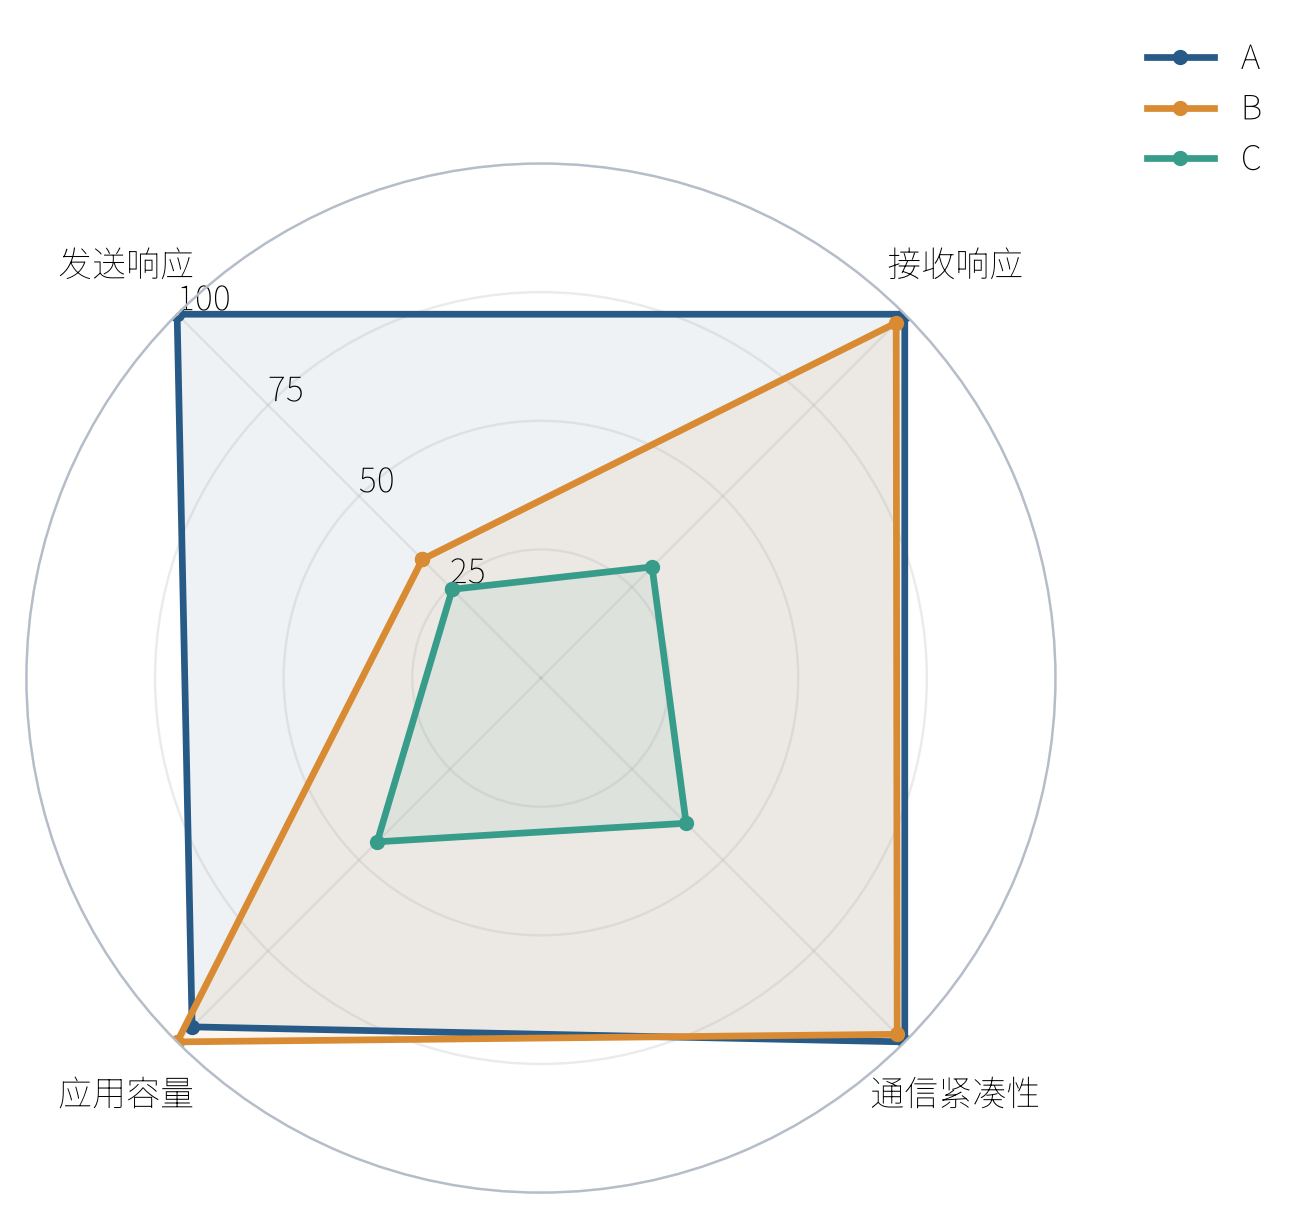
\includegraphics[width=.78\textwidth]{figures/representative-profile.png}
\caption{三组代表的归一化使用特征；分值越高表示对应指标越有利}
\label{fig:representative-profile}
\end{figure}

\section{三组代表的应用定位}

\subsection{A组：低延迟定向消息}

A组采用LATTE-3与BNN／ML-DSA-44。其重复加密和解密均处于亚秒级，适合需要交互响应的机构
消息、浏览器演示和频繁的小消息收发。ML-DSA组件具有固定标准对象格式，认证转换也便于复用
普通签名实现。A组的主要通信开销来自一次性认证而不是IBS签名，因此后续优化重点是外层认证
结构和整包长度。

\subsection{B组：原生模格身份认证与紧凑状态}

B组采用LATTE-3与SRGG PARAM-I。其接收端时间与A接近，主要额外成本集中在发送者发钥和
签名。范围感知编码显著减少SRGG主状态、用户密钥和签名长度。该组适合发送端能够承担数秒签名、
接收端需要快速验证的批量定向投递，也适合研究原生模格IBS和紧凑对象在完整协议中的作用。

\subsection{C组：固定身份对的连续通信}

C组采用Lai C2与Sageloli PARAM-I。初次解密需要完成高成本叶钥委派，密文也明显大于A、B；
建立接收会话后，同一身份对的后续解密不再重复委派。因而，C组更适合双方身份固定、允许离线
准备并连续处理多条消息的使用方式，例如固定管理端与受控终端之间的周期消息。其价值在于展示
高成本HIBE与环格IBS如何通过结构化采样和会话复用进入完整系统，而不是作为低延迟基线。

\section{本章小结}

本章说明了两种HIBE与六种IBS的算法关系和实现对象，并区分十种常规组合与LATTE＋Wang--PW
目标参数组合。A、B、C三组分别代表低延迟认证转换、原生模格身份签名和固定身份对的高成本
环格路线。下一章集中展开Sageloli采样、SRGG编码和Lai会话三项关键优化。

\chapter{关键算法优化}

第四章介绍的算法后端在结构、参数和对象规模上差异明显。直接照搬数学定义虽然可以描述算法，
却不能解决目标参数运行时出现的内存、存储和重复计算问题。本章围绕三个实际瓶颈展开：
Sageloli相关扰动不能展开为稠密矩阵，SRGG参考对象存在较大的文本表示开销，Lai在固定身份对
通信中会反复生成相同叶密钥。三项优化分别改变计算组织、对象编码和运行时生命周期，但不改变
原方案的公开方程与公共协议接口。

\section{Sageloli结构化环采样优化}

\subsection{稠密矩阵展开的资源瓶颈}

Sageloli的身份发钥和签名都需要在格陪集中采样。相关扰动由陷门决定其形状，再与离散采样
结合，生成满足方程和范数要求的短向量。环元素本来以多项式系数表示，乘法可以直接在
负循环环上计算；若把每个环元素展开为旋转矩阵，陷门和协方差会随之变成规模很大的实数矩阵。

PARAM-I取$d=2048$、$\ell=132$、$k=65$，签名相关扰动的系数维数为
\[
 D=d(\ell+k)=403456.
\]
仅显式保存一个$D\times D$双精度实数矩阵就需要约1.18~TiB，还没有计入矩阵分解和临时工作区。
这一数量超过常规工作站的可用内存，因此优化的重点不是减少常数，而是避免形成该矩阵。

实现始终保留多项式结构。公钥、主陷门和身份陷门分别以$\ell\times d$、
$(\ell-k)\times k\times d$和$\ell\times k\times d$的系数数组保存，环乘法在原环上执行。
每次发钥和签名结束后仍以精确整数算术检查
\[
 A=[\bar A\mid g-\bar AR],\qquad
 AT_s=H_1(P,\rho,s)-g\pmod q,
\]
因此改变的是内部计算方式，而不是密钥关系和验签条件。

\subsection{逐频率低秩分解}

设当前陷门为$T$，其形状为$\ell\times k$个环元素，并令
\[
 J=\begin{bmatrix}-T\\I_k\end{bmatrix},\qquad
 a=s^2-r^2,\qquad c=9r^2.
\]
相关扰动所需协方差为
\[
 \Sigma=aI-cJJ^\star,
\]
其中$\star$表示环上的伴随。$aI$是标量矩阵，修正项由只有$k$列的$J$生成，因而可以把主要
分解限制在低维子空间。

首先对多项式执行负循环Fourier变换。在每个频率$\nu$上，环乘法变为复数乘法，$J$对应
$(\ell+k)\times k$复矩阵$J_\nu$。随后计算
\[
 G_\nu=J_\nu^*J_\nu
      =U_\nu\operatorname{diag}(\lambda_i)U_\nu^*.
\]
在PARAM-I中，每个频率上需要分解的最大矩阵为$65\times65$，而不是$403456\times403456$。

\begin{figure}[H]
\centering
\begin{tikzpicture}[node distance=8mm and 7mm]
 \node[flow,text width=39mm] (poly) {陷门多项式$T$\\保存系数数组};
 \node[flow,text width=39mm,right=of poly] (fourier) {负循环Fourier变换\\$J_\nu$：$197\times65$};
 \node[flow,text width=39mm,right=of fourier] (gram) {计算$J_\nu^*J_\nu$\\分解$65\times65$矩阵};
 \node[check,text width=39mm,below=of gram] (apply) {对新随机向量应用\\低秩平方根};
 \node[check,text width=39mm,left=of apply] (inverse) {逆变换回系数域\\逐系数离散采样};
 \node[check,text width=39mm,left=of inverse] (verify) {检查精确模方程\\和原方案范数条件};
 \draw[flowarrow](poly)--(fourier);
 \draw[flowarrow](fourier)--(gram);
 \draw[flowarrow](gram)--(apply);
 \draw[flowarrow](apply)--(inverse);
 \draw[flowarrow](inverse)--(verify);
\end{tikzpicture}
\caption{Sageloli结构化相关扰动的计算流程（矩阵形状对应PARAM-I）}
\label{fig:ring-sampler}
\end{figure}

根据小矩阵的特征分解构造平方根算子
\[
 L_\nu=\sqrt a I-
 J_\nu U_\nu\operatorname{diag}\!\left(
 \frac{c}{\sqrt a+\sqrt{a-c\lambda_i}}
 \right)U_\nu^*J_\nu^*.
\]
该算子满足$L_\nu L_\nu^*=aI-cJ_\nu J_\nu^*$。应用算子时按右侧的小矩阵与向量乘法逐步
计算，不形成完整$L_\nu$。逆变换回系数域后，继续执行原方案要求的离散Gaussian和三进制
陪集采样。该方法沿用格陷门采样中的扰动思想\cite{micciancio2012trapdoors}，并针对当前
方案的环结构组织计算。

主要存储量由陷门系数和逐频率小矩阵计划组成，规模为$O(d\ell k+dk^2)$，不再随$D^2$增长。
同一陷门下可以复用已完成的数值计划，但每次发钥和签名仍使用新的随机样本。

\subsection{数值采样与精确代数校验}

Fourier变换和特征分解使用数值运算，方案中的模方程则必须精确成立。实现将两类职责分开：
数值计划在建立时检查正定充分条件和变换误差；回到系数域后，以整数算术检查环方程。大模数
$q=3^k$的公开乘积使用FLINT整数多项式，私有小整数乘法采用双素数NTT与CRT恢复，并检查
整数卷积幅度处于可唯一恢复范围。

签名生成后继续执行原方案的范数门和验签方程。浮点计算负责生成相关扰动，精确算术负责确认
最终代数关系。第七章给出PARAM-I、PARAM-II的实测时间、峰值内存及验签结果。

\section{SRGG对象的范围感知编码}
\label{sec:srgg-codec}

\subsection{参考表示的空间开销}

SRGG的公钥、陷门和签名包含大量多项式系数。JSON会把每个整数写成十进制字符串，并重复保存
负号、逗号、括号和字段名。对于大对象，这些语法字符和文本数字会形成显著的额外开销。

紧凑编码依据各字段的数学取值范围选择位数。例如，取值为$-1,0,1$的陷门系数只有三种可能，
每项用2~bit即可表示；公开模$Q=15744063$的系数位于$[0,Q)$，每项使用24~bit。短密钥和
签名响应先以Zigzag映射处理符号，再选择能够容纳该字段的最小统一位宽。

\begin{table}[H]
\centering\small
\caption{SRGG不同字段的紧凑编码方法}
\label{tab:codec-fields}
\begin{tabularx}{\textwidth}{@{}p{.23\textwidth}p{.25\textwidth}X@{}}
\toprule
\rowcolor{black!8} 数据 & 存储方法 & 解码时检查 \\
\midrule
公开模$Q$系数 & 每系数24~bit & $0\leq x<Q$ \\
三值陷门系数 & 每系数2~bit & 拒绝第四个未使用码字 \\
短密钥、响应整数 & Zigzag与最小统一位宽 & 数值范围、位宽最小性 \\
二元挑战 & 每系数1~bit & 固定多项式次数与长度 \\
类型、参数与上下文 & 固定头部和长度前缀 & 对象类别、公钥和参数一致 \\
\bottomrule
\end{tabularx}
\end{table}

对包含$N$个系数、统一位宽为$b$的字段，主体长度为$\lceil Nb/8\rceil$字节，再加必要头部。
解码后得到与JSON格式相同的数学对象，签名与验证仍调用原算法。

\subsection{四类对象的规范编解码}

范围感知编码同时用于公钥、主状态、用户密钥和签名。四类对象使用独立类型标识，系数顺序固定，
末字节中未使用的位必须为零。解析器先根据参数和形状计算预期长度，再读取数据，并检查对象类型、
身份、公钥上下文和系数范围。解码后重新编码必须得到相同字节串，从而排除同一数学对象的多种
字节表示。

对象变短可以减少密钥文件和传输字节，但收益取决于对象在完整协议中的占比。例如，IBS签名
变短会直接减少对称加密载荷，而HIBE胶囊和一次性认证仍构成固定开销。第七章同时报告四类对象
的JSON与紧凑格式长度、编解码时间以及完整密文组成，以区分对象级收益和协议级收益。

\section{Lai接收会话优化}
\label{sec:lai-session}

\subsection{固定身份对下的重复委派}

在Lai组合中，接收者持有第一层密钥$\mathsf{dk}_r$。解密来自发送者$s$的消息前，需要运行
\[
 \mathsf{dk}_{r,s}\leftarrow\mathsf{Derive}(\mathsf{dk}_r,s).
\]
同一接收者连续读取同一发送者的消息时，委派输入保持不变，逐消息生成叶钥会重复支付相同的
计算成本。与此同时，每条消息的HIBE胶囊、对称密文和IBS签名都不同，仍须逐条认证与解密。

作品引入显式接收会话：会话建立时生成并验证一次叶钥，随后在固定双方身份下复用。图
\ref{fig:receiver-session}对比两种计算安排。

\begin{figure}[H]
\centering
\begin{tikzpicture}[node distance=6mm and 6mm]
 \node[font=\small,anchor=east] (old) {逐条委派};
 \node[flow,right=of old,text width=30mm] (o1) {委派＋解密1};
 \node[flow,right=of o1,text width=30mm] (o2) {委派＋解密2};
 \node[flow,right=of o2,text width=30mm] (o3) {委派＋解密3};
 \node[font=\small,anchor=east,below=22mm of old] (new) {接收会话};
 \node[check,right=of new,text width=30mm] (prep) {委派一次\\验证并保留叶钥};
 \node[check,right=of prep,text width=30mm] (dec) {解密1、2、3\\逐条认证与验签};
 \node[check,right=of dec,text width=30mm] (close) {关闭会话\\停止使用叶钥};
 \draw[flowarrow](o1)--(o2);
 \draw[flowarrow](o2)--(o3);
 \draw[flowarrow](prep)--(dec);
 \draw[flowarrow](dec)--(close);
\end{tikzpicture}
\caption{Lai接收会话将与密文无关的委派移至准备阶段}
\label{fig:receiver-session}
\end{figure}

\subsection{身份绑定与会话生命周期}

会话建立时先检查公开上下文、接收者身份和一级密钥绑定；生成叶钥后再检查完整$(r,s)$路径及
陷门方程。会话只服务于当前公钥和身份对，关闭后停止解密。每条消息继续执行规范解析、外层字节
认证、HIBE解封装、AES-GCM验证、IBS验签和一次性公钥承诺核对。

叶钥作为秘密状态仅保留在进程内，会话对象不支持序列化；长期保存的接收密钥继续采用原有持久
格式。该边界避免为了性能而增加新的长期密钥文件，同时明确会话优化适用于双方身份固定的连续
通信。

\subsection{连续消息的摊销成本}

设一次会话准备耗时为$T_{\rm prep}$，会话内单条解密耗时为$T_{\rm sess}$。处理$N$条消息的
总成本和平均成本分别为
\[
 T_{\rm total}(N)=T_{\rm prep}+NT_{\rm sess},\qquad
 \bar T(N)=\frac{T_{\rm prep}}{N}+T_{\rm sess}.
\]
首条消息承担全部准备成本，消息数量增加后该成本逐渐摊薄。第七章把原路径解密、会话准备、
后续解密和叶钥内存分别列出，说明该优化的适用条件和代价。

\section{本章小结}

三项优化分别针对不可承受的中间矩阵、冗长的对象表示和固定身份对下的重复委派。Sageloli优化
通过逐频率低秩分解避免$O(D^2)$稠密表示；SRGG优化按字段范围建立规范二进制编码；Lai优化以
受身份和公钥约束的会话复用叶密钥。它们都保留原算法方程与通用协议接口，具体效果在第七章以
实测数据验证。

\chapter{软件系统与操作流程}

密码原语解决具体数学问题，软件系统还要负责组合选择、参数检查、对象保存和用户操作。本章
介绍系统怎样把后端、公共协议和应用入口分开，以及新增HIBE或IBS时需要完成哪些工作。

\section{分层软件架构}

系统自下而上分为基础设施层、密码原语层、组合层、协议层和应用层。基础设施层提供规范编码、
随机源、域分隔哈希、错误类型和原子文件保存。密码原语层分别实现HIBE和IBS。组合层根据配置
选择后端，并在生成密钥前完成能力与容量检查。协议层实现第三章的五个IB-ME算法。最上层提供
命令行、实验工具和浏览器演示。

\begin{figure}[H]
\centering
\begin{tikzpicture}[node distance=7mm and 8mm]
 \node[flow,text width=92mm] (web) {应用层：浏览器、CLI、实验工具};
 \node[flow,below=of web,text width=92mm] (protocol) {协议层：IB-ME五算法、Hybrid、字节认证};
 \node[check,below=of protocol,xshift=-27mm,text width=38mm] (assembly) {组合层\\SuiteConfig、注册表、预检};
 \node[check,below=of protocol,xshift=27mm,text width=38mm] (state) {状态层\\固定发钥、对象保存、恢复};
 \node[flow,below=of assembly,text width=38mm] (hibe) {HIBE后端\\LATTE、Lai};
 \node[flow,below=of state,text width=38mm] (ibs) {IBS后端\\六种签名实现};
 \node[check,below=of protocol,yshift=-48mm,text width=92mm] (core) {基础设施：规范编码、随机源、哈希、错误处理};
 \draw[flowarrow](web)--(protocol);
 \draw[flowarrow](protocol)--(assembly);
 \draw[flowarrow](protocol)--(state);
 \draw[flowarrow](assembly)--(hibe);
 \draw[flowarrow](state)--(ibs);
 \draw[flowarrow](hibe)--(core);
 \draw[flowarrow](ibs)--(core);
\end{tikzpicture}
\caption{软件系统的分层结构}
\label{fig:system-structure}
\end{figure}

这一结构有两个直接作用。第一，公共协议不根据算法名称编写分支。它只调用接口，并从组合配置
读取容量和格式。第二，应用入口不直接操作陷门、矩阵或多项式；命令行和浏览器收到的都是统一
角色对象和密文字节。因此，同一套页面、状态管理和错误处理可以服务不同组合。

\section{稳定的原语接口}

HIBE后端提供五个密码方法，IBS后端提供四个密码方法和一个签名加载方法。表
~\ref{tab:backend-interfaces}列出接口及其返回对象。

\begin{table}[H]
\centering\small
\caption{HIBE与IBS后端接口}
\label{tab:backend-interfaces}
\begin{tabularx}{\textwidth}{@{}p{.16\textwidth}p{.2\textwidth}X@{}}
\toprule
\rowcolor{black!8} 后端 & 方法 & 公共含义 \\
\midrule
HIBE & $\mathsf{setup}$ & 建立公开参数与主秘密 \\
HIBE & $\mathsf{extract}$ & 为第一层接收身份生成密钥 \\
HIBE & $\mathsf{derive}$ & 为第二层发送身份委派叶密钥 \\
HIBE & $\mathsf{encrypt}$ & 沿两层身份路径加密固定长度种子 \\
HIBE & $\mathsf{decrypt}$ & 用叶密钥恢复种子或返回拒绝 \\
\midrule
IBS & $\mathsf{setup}$ & 建立签名公开参数与主秘密 \\
IBS & $\mathsf{key\_extract}$ & 为发送身份生成签名密钥 \\
IBS & $\mathsf{sign}$ & 签署规范协议消息 \\
IBS & $\mathsf{verify}$ & 以公开参数、身份和消息验签 \\
IBS & $\mathsf{load\_signature}$ & 从规范字节恢复签名对象 \\
\bottomrule
\end{tabularx}
\end{table}

每种公开参数、主秘密、用户密钥、密文和签名都实现规范的$\mathsf{to\_bytes}$与
$\mathsf{from\_bytes}$。对象头包含类别、版本和参数摘要。后端加载对象时检查字段数量、长度、
数值范围和公开上下文，公共层无需了解其中的系数排列。

接口也明确随机源的传递方式。建立、发钥、加密和随机化签名从上层取得密码学随机源；验签与
规范解码不读取随机数。测试可以注入可重复随机流，正常运行使用操作系统随机源。同一方法在
不同入口下因此保持相同的随机性边界。

\section{组合配置与接入流程}

\subsection{完整组合配置SuiteConfig}

一套运行配置由$\mathsf{SuiteConfig}$描述。它记录HIBE与IBS选择器、算法版本、两边参数档、
密钥和签名格式、外部身份长度、混合载荷预算以及协议版本。配置使用排序字段和规范JSON编码，
其摘要进入公开对象和所有角色密钥。

注册表为每个后端保存四类信息：构造函数、参数预设、对象解码器和能力声明。能力声明包括
两层身份支持、内部身份宽度、直接明文容量、IBS输入上限、签名尺寸上界、所需运行依赖和允许的
编码格式。发现后端和查看配置只读取这些静态信息，不生成密钥。

运行前的$\mathsf{validate\_suite}$依次完成：
\begin{enumerate}
  \item 解析HIBE与IBS选择器，固定精确版本和参数档；
  \item 检查HIBE支持两层身份，外部身份编码后不超过内部上限；
  \item 计算IBS签名输入开销和最大应用消息长度；
  \item 检查签名上界与应用消息能够放入混合载荷预算；
  \item 检查对象格式和运行依赖，生成完整配置摘要。
\end{enumerate}
只有配置通过以后，系统才进入$\mathsf{Setup}$。容量不足会在昂贵建立之前给出所需字节数和
现有预算，用户可以选择更大载荷预算或另一后端。

\subsection{新增HIBE或IBS的接入步骤}

接入新HIBE时，实现者完成五个HIBE方法和五类对象，声明两层身份宽度、种子容量和参数预设，
再向注册表提供一个后端描述。接入新IBS时，实现四个密码方法、签名加载和四类对象，声明身份、
签名输入及签名输出上限。公共协议、Hybrid、BYTEAUTH、状态文件和应用入口均不修改。

\begin{figure}[H]
\centering
\begin{tikzpicture}[node distance=7mm and 7mm]
 \node[flow,text width=36mm] (alg) {实现论文算法\\与严格对象};
 \node[flow,right=of alg,text width=36mm] (cap) {声明参数、容量\\和编码格式};
 \node[flow,right=of cap,text width=36mm] (reg) {注册BackendSpec\\获得SuiteConfig};
 \node[check,below=of cap,text width=38mm] (unit) {原语正例、错身份\\篡改与恢复测试};
 \node[check,left=of unit,text width=38mm] (combo) {与现有另一类原语\\完成组合测试};
 \node[check,right=of unit,text width=38mm] (app) {沿用CLI与Web\\完成实际收发};
 \draw[flowarrow](alg)--(cap);
 \draw[flowarrow](cap)--(reg);
 \draw[flowarrow](reg)--(unit);
 \draw[flowarrow](unit)--(combo);
 \draw[flowarrow](unit)--(app);
\end{tikzpicture}
\caption{新增密码后端的接入过程}
\label{fig:new-backend}
\end{figure}

以Wang--PW为例，新增代码位于独立IBS目录，向外暴露与Sageloli、SRGG相同的方法。注册描述声明
目标档$s0$-4、393,320字节签名和4,096字节签名输入上限。组合层据此算出3,924字节应用容量，
并把混合载荷预算提高到能够容纳该签名的范围。随后直接复用LATTE、五个IB-ME算法、命令行角色
导入和错误输入流程，公共协议中没有新增“如果是Wang则……”的分支。

这一接入方式也是“通用设计”的软件依据。更换算法需要完成新原语本身及其元数据，而不是复制
一套IB-ME实现。十种常规配对和LATTE＋Wang--PW都经过同一入口形成。

\section{固定发钥与持久状态}

现实系统不会为每条消息重新建立主密钥。发钥机构需要长期保存主状态，并保证同一身份能够取回
先前发布的密钥。作品为HIBE接收者和IBS发送者分别维护发钥记录。

一次发钥分为准备、生成和提交三个阶段。准备阶段取得本地锁并写入待处理身份；生成阶段调用
底层原语；提交阶段先原子保存更新后的主状态，再发布用户密钥。若进程在生成中断，恢复程序会
看到待处理记录并停止继续发钥，避免同一身份在状态不明时获得第二份对象。

加载状态时，系统按图~\ref{fig:state-recovery}检查组合配置、公开上下文、参数快照、对象类型和
身份绑定。后端随后检查自己的代数关系，例如LATTE叶钥方程、SRGG对象形状或Wang--PW的
$AX+H_1=G$关系。通过后才恢复运行实例。

\begin{figure}[H]
\centering
\begin{tikzpicture}[node distance=8mm and 8mm]
 \node[flow,text width=34mm] (files) {读取公开对象\\主状态与角色密钥};
 \node[flow,right=of files,text width=34mm] (codec) {规范解码\\版本与长度检查};
 \node[flow,right=of codec,text width=34mm] (bind) {配置摘要、身份\\公开参数绑定};
 \node[check,below=of codec,text width=40mm] (math) {后端代数关系与状态账本检查};
 \node[check,left=of math,text width=36mm] (runtime) {恢复运行实例\\继续加密或解密};
 \draw[flowarrow](files)--(codec);
 \draw[flowarrow](codec)--(bind);
 \draw[flowarrow](bind)--(math);
 \draw[flowarrow](math)--(runtime);
\end{tikzpicture}
\caption{持久对象恢复流程}
\label{fig:state-recovery}
\end{figure}

公开对象、发送密钥、接收密钥和密文可以分别导出。角色导入只要求该角色实际需要的对象：
发送端不读取HIBE主秘密，接收端不读取IBS主秘密。这样可以在不同进程甚至不同主机上执行发送
和接收，同时保持相同的组合配置与编码。

\section{命令行与浏览器操作}

命令行适合批量实验、持久状态和跨进程恢复。典型流程为：选择组合并建立系统；为Alice、Bob
导出角色密钥；Alice指定Bob并加密；Bob指定Alice并解密；关闭进程后重新导入对象，再次解密
已有密文。实验驱动在此基础上记录每阶段时间、对象字节数和进程树RSS。

浏览器界面使用同一运行时，不另写一套密码代码。使用者首先选择组合，然后输入接收者、发送者、
期望发送者和消息。页面显示建立、发钥、签名、封装和解密阶段，并展示密文长度、耗时和最终
结果。对于耗时较长的B组，任务在服务端继续执行，页面刷新后可以重新连接正在运行的任务。

\begin{figure}[H]
\centering
\includegraphics[width=.98\textwidth]{../../deliveries/2026-10-20-web-redesign/desktop.png}
\caption{A组实际收发界面：指定双方身份、加密消息与匹配解密}
\label{fig:web-demo}
\end{figure}

图~\ref{fig:web-demo}记录A组的一次实际操作：Alice向Bob发送36字节UTF-8消息，Bob选择Alice为
期望发送者后恢复原文。A、B还分别在同一条密文上执行三种身份错配、翻转1 bit和截短1字节，
均得到拒绝。两组该次密文长度分别为142,095字节和149,255字节。

\section{运行优化与部署方式}

除了第五章的三项主要优化，系统还减少两类重复工作。BNN签名包含机构证书和用户消息签名。对
同一身份的连续消息，系统缓存“证书已经验证”的公开结果，但每条消息仍重新验证用户签名。
缓存绑定完整证书、用户公钥和身份，并使用有界LRU管理。

SRGG签名的一部分数值准备只取决于固定签名密钥和数值选项。实现可以复用该计划，每条签名仍
重新生成随机量。实验表明这两类局部缓存对完整流程的影响小于结构化采样、紧凑编码和Lai会话，
因此它们作为运行细节保留。

系统支持单机演示和分角色部署。单机模式把发钥机构、发送端、接收端和浏览器服务放在一台主机，
便于比赛现场操作。分角色模式由发钥机构离线生成角色对象，发送端和接收端分别导入自己的密钥；
密文可通过任意字节传输通道送达。

\begin{figure}[H]
\centering
\begin{tikzpicture}[node distance=9mm and 12mm]
 \node[check,text width=38mm] (issuer) {发钥机构\\建立系统、签发角色密钥};
 \node[flow,below left=of issuer,text width=36mm] (sender) {发送端\\导入公开对象与发送密钥};
 \node[flow,below right=of issuer,text width=36mm] (receiver) {接收端\\导入公开对象与接收密钥};
 \node[check,below=of issuer,yshift=-34mm,text width=38mm] (channel) {公开传输通道\\只传递规范密文};
 \draw[flowarrow](issuer)--node[left,font=\small]{发送角色对象}(sender);
 \draw[flowarrow](issuer)--node[right,font=\small]{接收角色对象}(receiver);
 \draw[flowarrow](sender)--(channel);
 \draw[flowarrow](channel)--(receiver);
\end{tikzpicture}
\caption{发钥机构、发送端与接收端的部署关系}
\label{fig:deployment}
\end{figure}

原生模块在创建适配器时会检查接口和二进制。已有部署对照发现，把安装包和运行文件放在Linux
本地文件系统可以减少跨挂载目录的重复读取。该调整不改变算法、参数和密文格式，第七章列出
同一运行时下的对照结果。

除主要实验机器外，项目还在Xeon Silver 4216主机的NixOS、Sage~10.9和Python~3.14.7环境
完成独立安装。A、B各执行25条操作，C完成匹配解密、内部签名拒绝和恢复。C最初因900秒阶段上限导致超时；
调整为3600秒后完成三个长阶段，耗时约21至27分钟。这次复现用于检查安装、对象恢复和完整调用路径；
性能分析仍采用第七章逐项列明的原始实验环境。

\section{本章小结}

软件系统通过稳定接口、组合配置和注册表把底层算法与公共协议分开。新增后端只实现自身算法、
对象与能力声明，随后即可复用五个IB-ME算法、状态管理、CLI和浏览器入口。固定发钥和规范恢复
使系统能够跨进程长期使用，单机与分角色部署则覆盖演示和实际通信两种方式。

\chapter{测试与结果分析}

\section{实验设置}
实验分别考察完整系统的运行成本、三项主要优化、部署改动和功能正确性。数学基础见第二章，
具体算法与参数见第四章；身份和消息采用规范字节编码，正常密码操作使用操作系统随机源。
不同实验的环境与重复方式集中列于表~\ref{tab:environments}。

\begin{table}[H]
\centering\small
\caption{主要实验环境与重复方式}
\label{tab:environments}
\begin{tabularx}{\textwidth}{@{}p{.18\textwidth}Xp{.29\textwidth}@{}}
\toprule
\rowcolor{black!8} 实验 & 环境 & 输入与重复 \\
\midrule
十组合同机比较 & Ultra 9 275HX，WSL2，Sage 10.9／Python 3.13.14，OMP 4、BLAS 1 & 身份各64 B，消息32 B；每组1个独立根，首次、重复与恢复各1次 \\
A/B多根重复 & i9-14900HX，WSL2，Sage 10.7／Python 3.12.13，OMP 4、BLAS 1 & 身份各64 B，消息32 B；每组独立建立3套系统，每套3对重复加解密 \\
Sageloli采样 & Ultra 7 255HX，WSL2，Python 3.13.15，OMP与BLAS均4 & PARAM-I、II各建立1套；身份21 B、消息33 B及后续消息 \\
SRGG编码 & Ultra 7 255HX，WSL2，Python 3.13.15，OMP与BLAS均1 & 每档3套系统；同对象交替测量两种编码各5次 \\
C阶段分解 & Ultra 9 275HX，WSL2，Sage 10.9／Python 3.13.14，OMP与BLAS均1 & 身份各64 B，消息32 B；C组合1次，解密进程存在并发 \\
接收会话 & 与A/B主实验的机器及运行时相同 & 1套系统；原解密2次，准备1次，会话解密3次 \\
部署位置 & Ultra 9 275HX，WSL2，Python 3.13.14，OMP 4、BLAS 1 & 相同3套状态；每种位置各30次完整加密、解密 \\
\bottomrule
\end{tabularx}
\end{table}

完整流程计时包含组合编码、对象检查和原语调用。首次解密包含叶钥生成；恢复实验另起进程加载
已有对象。十组合实验固定逻辑CPU~0--3，OpenBLAS、MKL与NUMEXPR均为1线程，首次操作在运行库
准备后开始计时。表中重复测量描述固定密钥下的运行波动，独立建立系统的数量单独列出。下文时间
通常保留3位有效数字；B、KiB、MiB分别表示字节、$2^{10}$字节和$2^{20}$字节。

\subsection{组合覆盖与代表方案}

第四章表~\ref{tab:implemented-matrix}已经列出两种HIBE与五种常规IBS形成的十种组合。测试阶段
对每一格都调用真实后端，完成系统建立、双方发钥、首次与重复消息收发、新进程恢复和外层篡改
拒绝。组合数量按底层算法计数，同一算法的不同参数档及参考／紧凑格式不重复计为新方案。

十种组合形成常规后端的主要横向比较；A、B、C在此基础上承担更深入的重复、阶段分解和专项优化
分析。Wang--PW是在常规十种组合之后接入的第六种IBS，目前完成LATTE＋Wang--PW目标档，
其输入长度、运行机器和资源规模不同，因而单独列出分阶段结果，不纳入十组合排序。

\subsection{评价指标}

实验按“离线准备、在线收发、持久恢复”三阶段记录。离线准备包括系统建立与双方发钥；在线
收发包括首次加密、首次解密和固定密钥下的重复操作；持久恢复另起进程加载公开对象与角色密钥。
时间采用墙钟时间，尺寸采用实际规范编码字节数，内存采用定期采样的进程树RSS峰值。

这些指标对应不同部署选择。发钥机构更关心Setup、KeyExtract和主状态，发送端更关心签名与
完整加密，接收端更关心叶钥委派和解密，网络侧则关心完整密文而不是单个签名。后文先分析
完整系统，再把总成本分解到具体优化。

\section{十种常规组合的同机基本比较}

\subsection{实验方法与完成情况}

十种组合使用同一份固定源码归档、相同原生引擎和依赖版本，按串行方式运行。三组来自同口径
预运行，另外七组在相同环境下补齐；两批的源码摘要、软件环境、线程设置和输入完全一致。每种
组合建立一个新的系统根，依次执行首次加解密、同进程重复加解密、新进程对象恢复和恢复后解密，
并分别检查密文截断和单比特翻转。这里的“十组”表示十种HIBE与IBS配对，不表示每组重复十次。

十种组合全部完成，共通过20次诚实加密、30次诚实解密、10次新进程恢复和20次外层拒绝，没有
失败记录。每项时间只有一个独立根上的一次观测，因此下文使用“实测值”，不计算中位数、误差线
或置信区间。所用配置均为第四章列出的目标或论文参数而非教学参数；哈希与随机预言机接口使用
SHAKE实例化，ROM或QROM适用范围沿用相应原语文献，功能与性能测试不替代安全性论证。

\subsection{首次完整流程时间}

表~\ref{tab:ten-first-times}按同一口径列出从系统建立到首次解密的五个阶段。系统建立和双方发钥
主要反映可信发钥机构的准备成本，首次加密与首次解密则包含完整协议编码、签名、HIBE封装、叶钥
生成和认证检查。

\begin{table}[H]
\centering\small
\caption{十种组合的首次完整流程实测时间，单位为秒}
\label{tab:ten-first-times}
\setlength{\tabcolsep}{4pt}
\begin{tabular}{@{}lrrrrr@{}}
\toprule
\rowcolor{black!8} 组合 & 建立 & 发送者发钥 & 接收者发钥 & 首次加密 & 首次解密 \\
\midrule
% BEGIN DATA ten-first-times.tex
LATTE＋ML-DSA & 0.729 & 0.0139 & 0.224 & 0.0129 & 0.103 \\
LATTE＋Falcon & 0.689 & 0.0229 & 0.34 & 0.0153 & 0.0951 \\
LATTE＋Luo & 0.819 & 1.64 & 0.37 & 0.974 & 0.2 \\
LATTE＋SRGG & 1.08 & 33.3 & 0.385 & 17.6 & 0.125 \\
LATTE＋Sageloli & 3.11 & 50.9 & 9.98 & 12.9 & 0.616 \\
Lai＋ML-DSA & 1.95 & 0.549 & 30.6 & 86.5 & 422 \\
Lai＋Falcon & 2.14 & 0.621 & 32 & 90.9 & 440 \\
Lai＋Luo & 2.14 & 0.8 & 31.2 & 85 & 427 \\
Lai＋SRGG & 2.26 & 28.1 & 30.7 & 91.2 & 428 \\
Lai＋Sageloli & 4.6 & 49.9 & 39.5 & 96.4 & 412 \\
% END DATA ten-first-times.tex
\bottomrule
\end{tabular}
\end{table}

LATTE与ML-DSA、Falcon组合的首次加密分别为12.9和15.3毫秒；更换为Luo、SRGG和Sageloli后，
首次加密分别为0.974、17.6和12.9秒，差异主要来自IBS发钥与签名路径。LATTE五组首次解密为
95.1至616毫秒，说明在接收HIBE不变时，IBS验证虽有影响，但不会改变整体量级。

Lai五组首次加密集中在85.0至96.4秒，首次解密集中在412至440秒。更换IBS后结果仍处于同一
量级，表明该配置下Lai封装与真实随机委派是在线收发的主要成本。Sageloli使发送者发钥进一步
增至约50秒，但其影响叠加在Lai的分钟级解密之上，不能仅看完整时间判断IBS自身代价。

\subsection{重复操作与新进程恢复}

图~\ref{fig:ten-combination-times}同时展示首次、同进程重复和恢复后操作。横轴采用对数尺度，以
容纳毫秒级LATTE认证转换组合和分钟级Lai组合；每个点对应一个独立根上的一次实测，不绘制并不
存在的统计误差线。

\begin{figure}[H]
\centering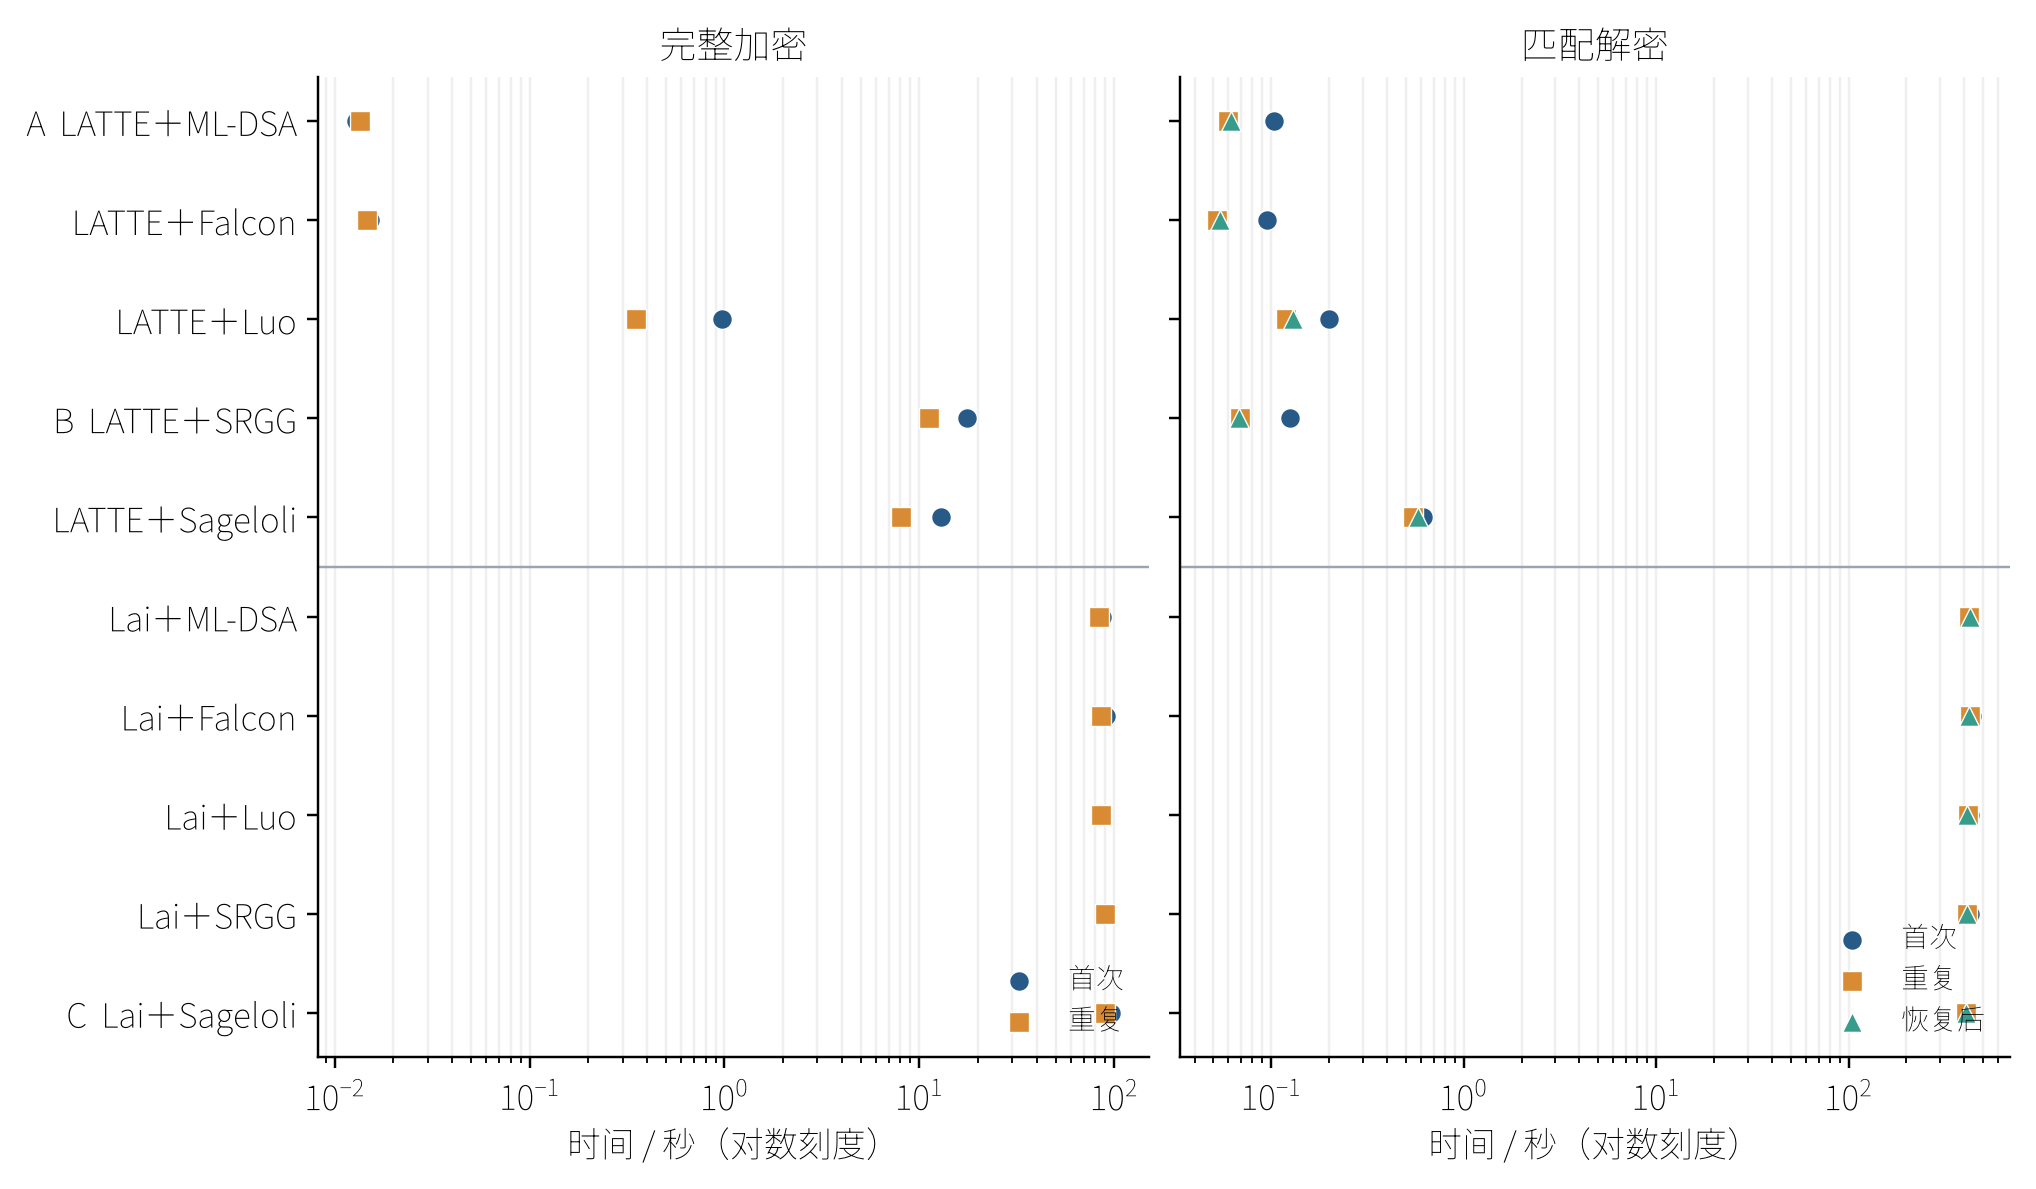
\includegraphics[width=.98\textwidth]{figures/ten-combination-times.png}
\caption{十种组合的首次、重复与恢复后完整操作时间；A、B、C为三组代表}
\label{fig:ten-combination-times}
\end{figure}

LATTE＋Luo、SRGG和Sageloli的重复加密分别降至0.351、11.3和8.04秒，与相同发送密钥下可以
复用部分数值准备的实现结构一致。LATTE五组恢复后解密为54.5至577毫秒，和同进程重复解密接近，
说明规范对象加载没有改变接收路径的量级。Lai五组恢复后解密仍为406至428秒，因为恢复不会缓存
新的随机委派结果；这与第五章另行讨论的“准备接收会话”是两种不同状态策略。

\subsection{规范对象尺寸与运行内存}

表~\ref{tab:ten-object-sizes}列出同一系统根产生的公共对象、主状态、双方角色对象和完整密文。
尺寸均取实际规范二进制编码长度，不使用数学对象的内存估算。

\begin{table}[H]
\centering\small
\caption{十种组合的规范对象与完整密文长度}
\label{tab:ten-object-sizes}
\setlength{\tabcolsep}{3.2pt}
\begin{tabular}{@{}lrrrrr@{}}
\toprule
\rowcolor{black!8} 组合 & 公共对象 & 主状态 & 发送钥 & 接收状态 & 完整密文 \\
\midrule
% BEGIN DATA ten-object-sizes.tex
LATTE＋ML-DSA & 14.1~KiB & 142~KiB & 7.86~KiB & 125~KiB & 139~KiB \\
LATTE＋Falcon & 13.7~KiB & 137~KiB & 4.1~KiB & 125~KiB & 135~KiB \\
LATTE＋Luo & 255~KiB & 479~KiB & 306~KiB & 125~KiB & 148~KiB \\
LATTE＋SRGG & 46.2~KiB & 231~KiB & 82.4~KiB & 125~KiB & 146~KiB \\
LATTE＋Sageloli & 3.36~MiB & 149~MiB & 137~MiB & 125~KiB & 3.21~MiB \\
Lai＋ML-DSA & 1.54~MiB & 3.86~MiB & 7.86~KiB & 19.5~MiB & 1.27~MiB \\
Lai＋Falcon & 1.54~MiB & 3.85~MiB & 4.1~KiB & 19.5~MiB & 1.27~MiB \\
Lai＋Luo & 1.78~MiB & 4.19~MiB & 306~KiB & 19.5~MiB & 1.28~MiB \\
Lai＋SRGG & 1.58~MiB & 3.95~MiB & 82.3~KiB & 19.5~MiB & 1.28~MiB \\
Lai＋Sageloli & 4.9~MiB & 153~MiB & 137~MiB & 19.5~MiB & 4.34~MiB \\
% END DATA ten-object-sizes.tex
\bottomrule
\end{tabular}
\end{table}

接收状态几乎完全由HIBE决定：LATTE五组约为125~KiB，Lai五组约为19.5~MiB。发送钥则主要由
IBS决定，同一种IBS分别搭配两种HIBE时长度基本一致。完整密文也呈现可分解的结构：固定IBS后，
由LATTE换为Lai会增加约1.192~MiB；采用Sageloli时，大型IBS签名又使完整密文达到3.21和
4.34~MiB。该规律与后文按字段核算密文组成的结果一致。

图~\ref{fig:ten-combination-resources}把完整密文与运行期间的最大采样RSS并列。除Sageloli外，
十组合各阶段最大采样RSS约为254至885~MiB；LATTE＋Sageloli约1.64~GiB，Lai＋Sageloli约
1.97~GiB。RSS每10毫秒采样一次，包含运行库与子进程，共享页可能重复计数，因而用于同批次资源
比较而不是精确物理内存分解。

\begin{figure}[H]
\centering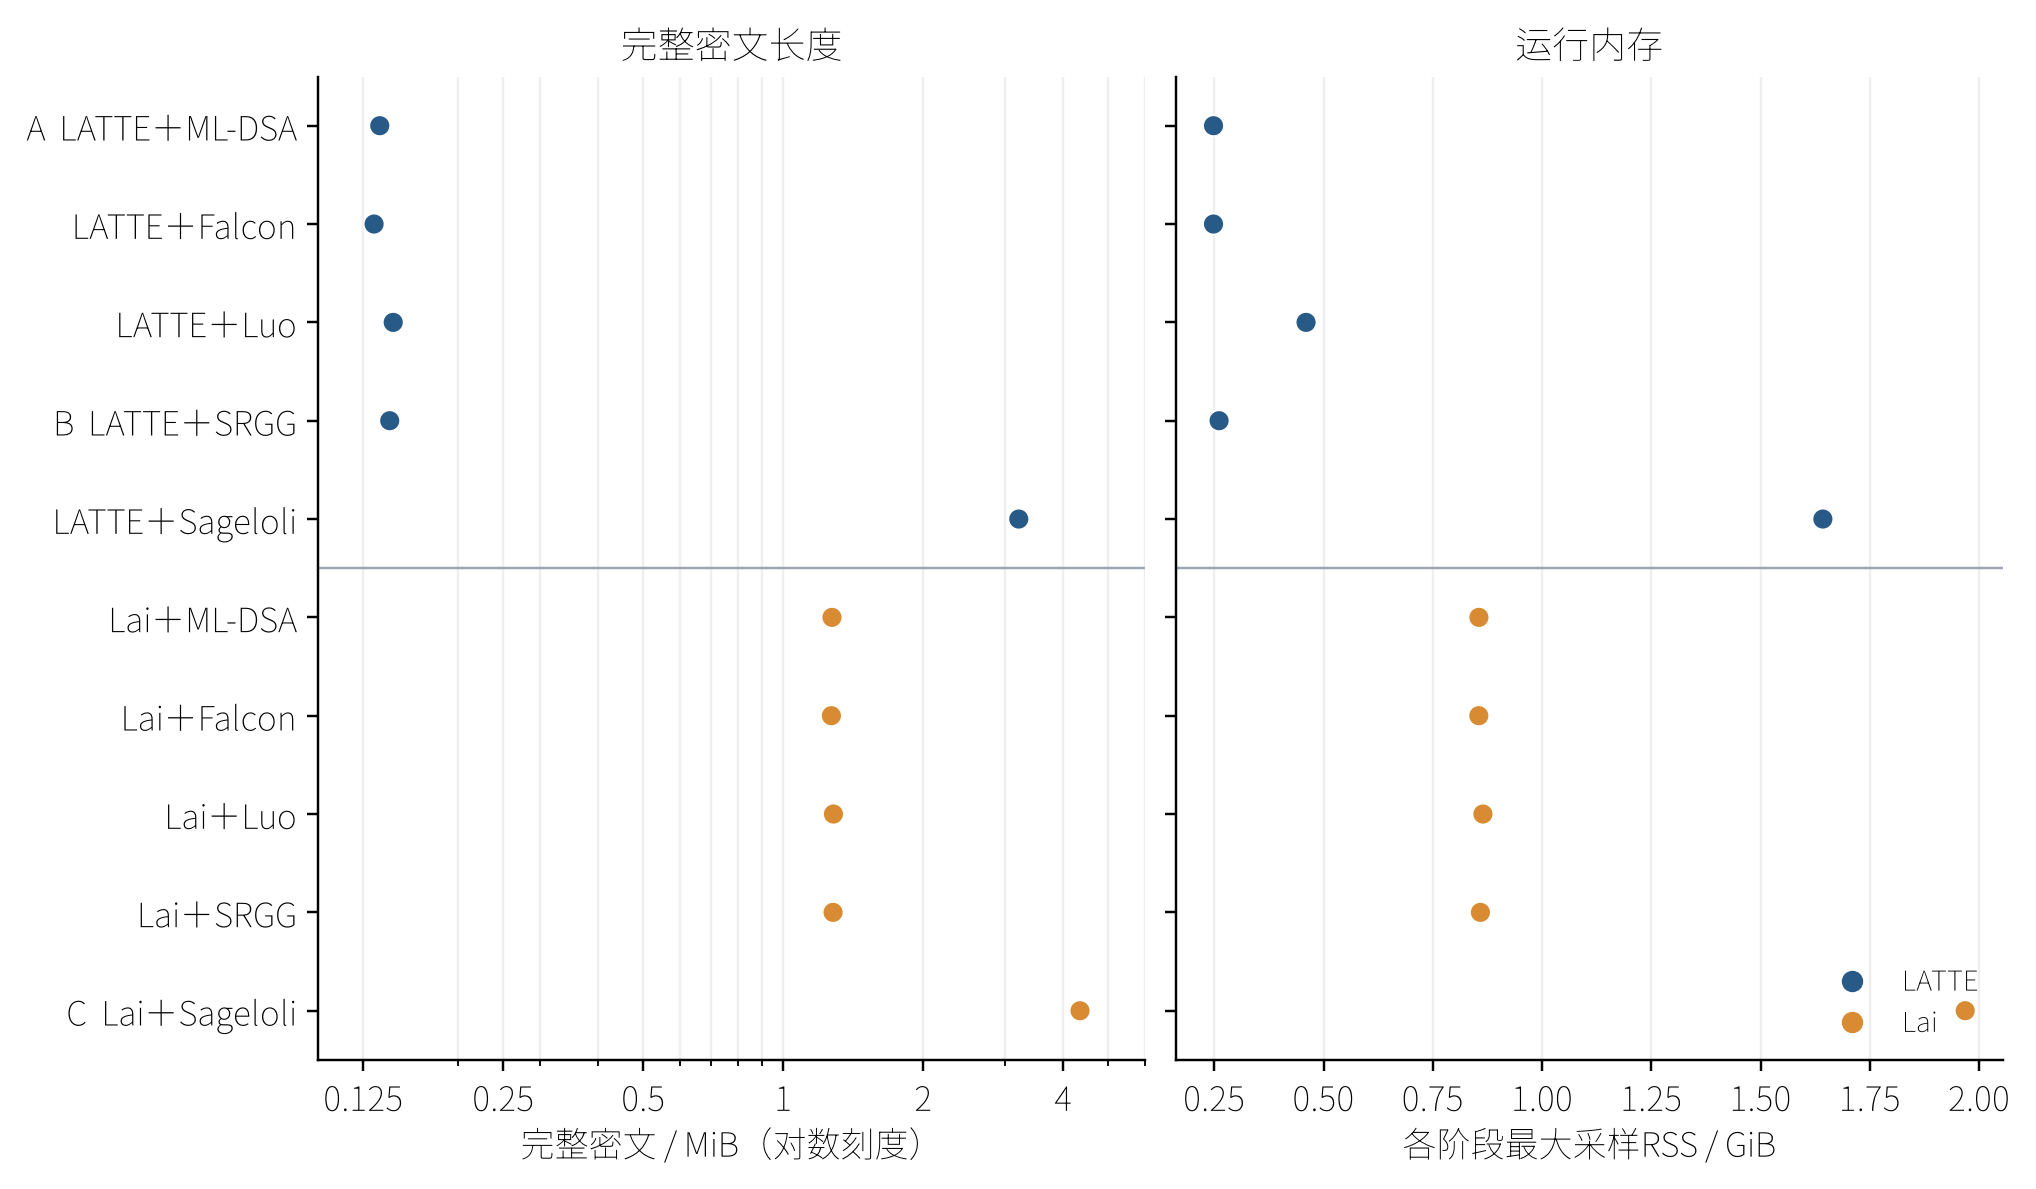
\includegraphics[width=.98\textwidth]{figures/ten-combination-resources.png}
\caption{十种组合的完整密文长度与各阶段最大进程树采样RSS}
\label{fig:ten-combination-resources}
\end{figure}

\subsection{组合差异与代表方案}

横向结果表明，HIBE和IBS影响完整系统的不同位置。HIBE主要决定接收状态、HIBE胶囊和解密委派；
IBS主要决定发送者发钥、签名生成、发送钥和签名字段。采用LATTE时，五种IBS的发送差异可以直接
观察；采用Lai时，HIBE成本占主导，但不同IBS仍通过密钥和密文长度体现。因而系统选型不宜把全部
指标压缩成单一总分，而应分别考虑发钥机构、发送端、接收端和网络侧资源。

三组代表由此对应三种明确用途。A提供低延迟标准化签名路径；B保留快速接收，同时展示原生模格
IBS和紧凑编码的发送端代价；C覆盖另一HIBE与环格IBS，并为结构化采样和固定身份对会话优化提供
完整对象。第四章的代表方案表采用本节同机数据，下面的多根与阶段实验继续回答运行波动和瓶颈
组成，而不再承担十组合横向排名。

\section{代表方案的重复与专项分析}
\subsection{A/B多根重复实验}
A、B使用相同LATTE参数与相同输入，主要差别在IBS。该批实验在另一台机器上分别建立3个独立
系统根，每根执行3次重复操作，用于观察固定组合的运行波动。表~\ref{tab:ab-times}给出完整生命
周期的中位时间，图~\ref{fig:ab-times}展示重复加解密的9次观测；这些值不与前述单根同机结果求
平均。

\begin{table}[H]
\centering\small
\caption{A/B完整流程中位时间，单位为秒}
\label{tab:ab-times}
\begin{tabular}{@{}lrrr@{}}
\toprule
\rowcolor{black!8} 操作 & A & B & 测量次数（A/B） \\
\midrule
% BEGIN DATA ab-timings.tex
系统建立 & 1.12 & 1.6 & 3/3 \\
发送者发钥 & 0.0954 & 32.1 & 3/3 \\
接收者发钥 & 0.427 & 0.457 & 3/3 \\
首次加密 & 0.0963 & 9.14 & 3/3 \\
首次解密 & 0.284 & 0.239 & 3/3 \\
重复加密 & 0.0785 & 9.17 & 9/9 \\
重复解密 & 0.152 & 0.161 & 9/9 \\
对象恢复 & 0.845 & 0.89 & 3/3 \\
恢复后解密 & 0.154 & 0.134 & 9/9 \\
% END DATA ab-timings.tex
\bottomrule
\end{tabular}
\end{table}

两组接收者发钥和重复解密接近，额外成本主要出现在B的发送者发钥与签名生成。A、B重复加密中位数分别为78.5毫秒和9.17秒，重复解密分别为152毫秒和161毫秒。A适合作为交互演示基线；B展示原生模块格IBS在同一完整协议中的运行特点。

\begin{figure}[H]
\centering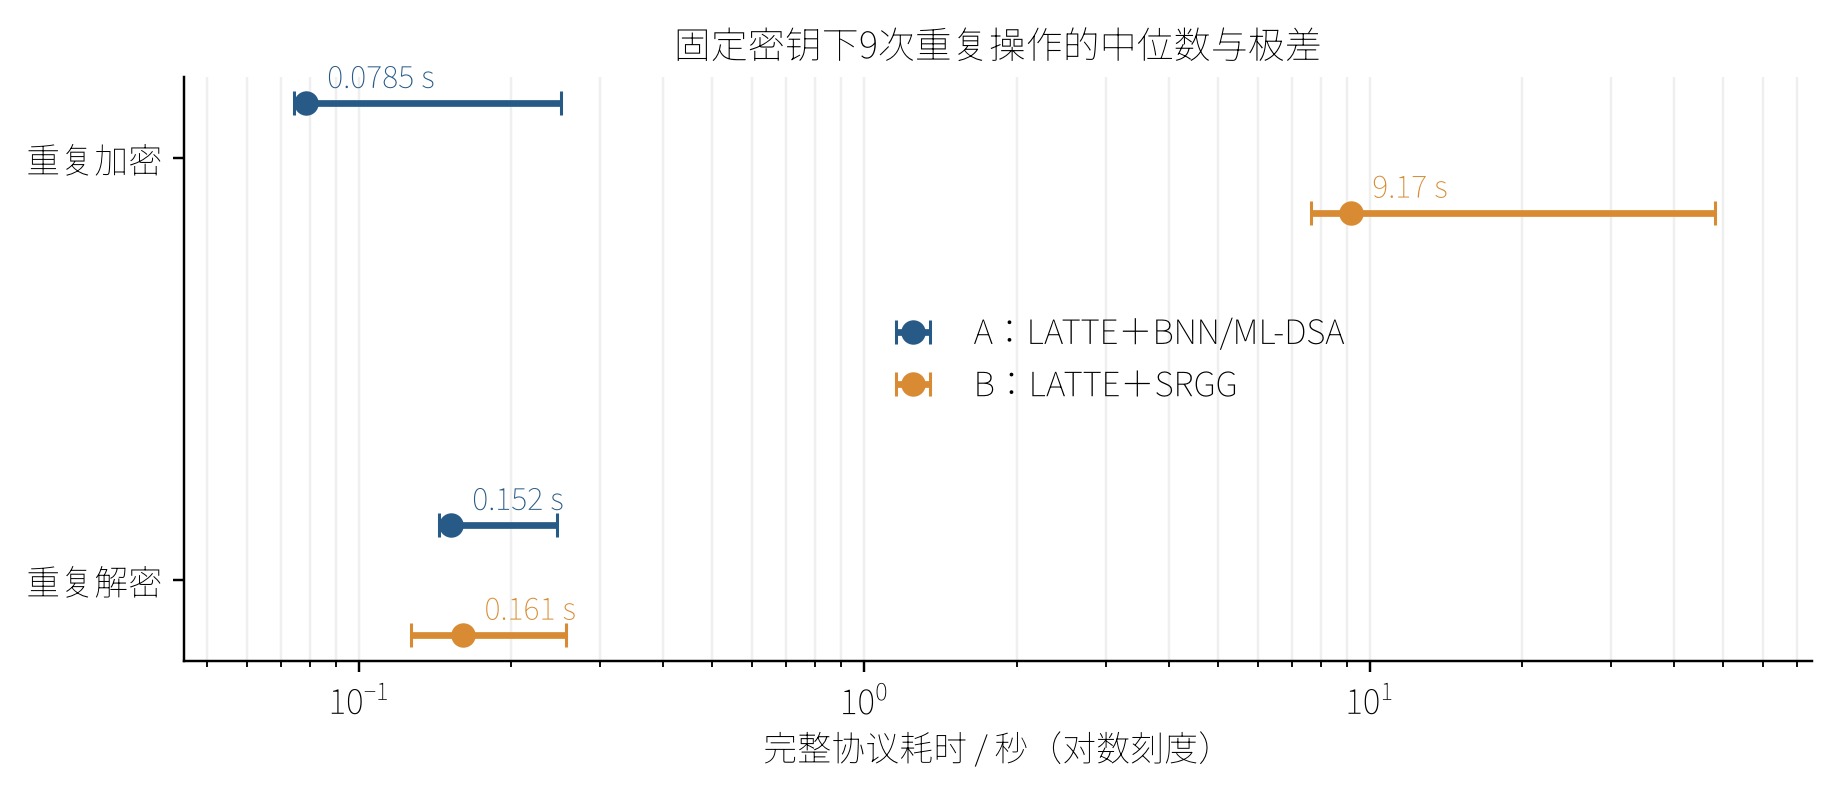
\includegraphics[width=.98\textwidth]{figures/ab-times.png}
\caption{A/B重复加密与解密时间。圆点为中位数，横线表示9次观测的最小值至最大值；横轴采用对数刻度}
\label{fig:ab-times}
\end{figure}

极差线显示了固定密钥下的运行波动。B有一次重复加密耗时约48.2秒，明显高于其中位数；A也有
较慢观测。首次解密包含叶钥生成，因此通常高于重复解密；恢复对象后，解密回到与重复操作相近
的量级。

\subsection{A/B多根实验的对象尺寸与内存}
表~\ref{tab:ab-sizes}汇总公共对象、主状态和双方密钥的编码长度。A、B完整密文约139 KiB和146 KiB；本章后面的密文组成分析进一步解释这些字节来自哪里。

\begin{table}[H]
\centering\small
\caption{A/B对象编码长度约值与运行内存}
\label{tab:ab-sizes}
\begin{tabular}{@{}crrrrrr@{}}
\toprule
\rowcolor{black!8} 组 & 公钥 & 主状态 & 发送钥 & 接收状态 & 完整密文 & 内存/MiB \\
\midrule
% BEGIN DATA ab-sizes.tex
A & 14 & 173 & 7.86 & 125 & 139 & 460 \\
B & 46.2 & 262 & 82.4 & 125 & 146 & 485 \\
% END DATA ab-sizes.tex
\bottomrule
\end{tabular}
\begin{minipage}{.96\textwidth}\footnotesize
前五项单位为KiB。对象长度按记录范围取近似值；内存为每10毫秒采样的进程树RSS最高值，包含运行库和子进程，短时峰值可能未被采样捕获。
\end{minipage}
\end{table}

B的公钥、主状态与发送钥大于A，接收状态接近，符合两组共用HIBE而采用不同IBS的结构。编码文件大小和运行内存分别统计：紧凑密钥文件加载后仍会恢复为数学对象，运行时还需要数值库、采样工作区和子进程。

\subsection{C组合的委派开销}
十组合主实验中，C的首次加密和解密分别为96.4秒和412秒。另一次保存了内部阶段的32字节消息
测试记录：加密99.0秒，匹配解密425秒，其中Lai委派为393秒，占约92.5\%。两次运行的条件和
目的不同，不能合并为重复样本，但都表明接收端的主要瓶颈是为认可发送身份生成叶钥。该阶段分解
记录的解密进程存在并发，因此只用于说明成本组成。

C的传输密文约4.34 MiB，大部分来自Sageloli签名和Lai胶囊。它展示了另一类HIBE与环IBS在论文配置下的完整组合，以及会话摊销的使用方式。下面分别分析通信量与准备成本。

\subsection{Wang--PW目标档的分阶段运行}

Wang--PW目标档使用$n=512$、$q=4294967291$和$s_0=4$。其密钥和采样工作区远大于常规组合，
因此在128~GiB级服务器上完成目标规模运行。表~\ref{tab:wang-results}汇总已经保存的建立、发钥、
独立签名和LATTE组合结果。

\begin{table}[H]
\centering\small
\caption{Wang--PW目标档与LATTE组合的实测结果}
\label{tab:wang-results}
\begin{tabularx}{\textwidth}{@{}p{.28\textwidth}rX@{}}
\toprule
\rowcolor{black!8} 项目 & 结果 & 说明 \\
\midrule
Setup & 536.63 s & 生成目标档公开矩阵和根陷门 \\
公开参数 & 67,109,371 B & 规范二进制对象 \\
主状态 & 603,980,295 B & 保存紧凑根陷门与参数 \\
KeyExtract & 5,431.95 s & 为一个64字节身份生成用户陷门 \\
用户签名密钥 & 2,214,593,131 B & 规范二进制对象 \\
独立Sign & 175.79 s、175.15 s & 两次恢复后的新消息签名均通过公开验签 \\
签名 & 393,320 B & 包含身份盐、消息盐和短原像 \\
签名峰值RSS & 约41.3 GiB & 进程树采样峰值 \\
LATTE＋Wang加密 & 192.54 s & 78字节应用消息，包含一次新Wang签名 \\
匹配解密 & 2.85 s & 从恢复的接收状态完成诚实解密 \\
完整密文 & 529,207 B & Hybrid与完整字节认证后的wire长度 \\
组合驱动总时长 & 254.86 s & 含准备、一次加密、诚实解密和错误输入检查 \\
\bottomrule
\end{tabularx}
\end{table}

目标档实验分阶段保存并复用已经生成的根和用户密钥。Setup、KeyExtract来自较早的目标生命周期，
最终两次签名与LATTE组合使用修订后的签名实现；表中按阶段呈现这些结果，不把它们相加成一次
连续生命周期。

从使用过程看，Setup和KeyExtract适合放在发钥机构的离线阶段。发送端一次签名约176秒，并需要
约41.3~GiB峰值内存，是组合加密的主要成本。接收端只进行公开验签与LATTE解封装，诚实解密约
2.85秒。393,320字节IBS签名进入对称载荷后，完整密文约517~KiB，明显小于用户签名密钥，
但仍高于A、B。

这一结果表明通用框架能够容纳大对象矩阵SIS后端，同时也说明它更适合低频签名、离线发钥和
资源充足的发送端。三组代表保持A、B、C不变，Wang--PW作为目标规模补充方案单独展示。

\section{完整密文的通信开销}
\subsection{完整密文的组成}
混合加密使应用消息不再受HIBE短明文容量直接限制，但种子胶囊、IBS签名和一次性认证仍需要传输。依据现有安装运行记录与实际编码格式，可将A的一条32字节消息和C的一条空消息分解为表~\ref{tab:ciphertext-parts}。

\begin{table}[H]
\centering\small
\caption{两条已有密文的字节组成核算}
\label{tab:ciphertext-parts}
\begin{tabular}{@{}lrr@{}}
\toprule
\rowcolor{black!8} 组成部分 & A：消息32 B & C：空消息 \\
\midrule
一次性公钥 & 65,536 & 65,536 \\
一次性签名 & 32,768 & 32,768 \\
IBS签名 & 6,237 & 3,227,824 \\
HIBE胶囊 & 37,088 & 1,228,844 \\
应用消息 & 32 & 0 \\
上下文、格式、nonce与标签 & 432 & 432 \\
\midrule
合计 & 142,093 & 4,555,404 \\
\bottomrule
\end{tabular}
\begin{minipage}{.96\textwidth}\footnotesize
整包长度来自已有运行；固定字段按序列化模块核算，HIBE胶囊长度由整包扣除其他组成得到。该核算没有新增加密实验。
\end{minipage}
\end{table}

\begin{figure}[H]
\centering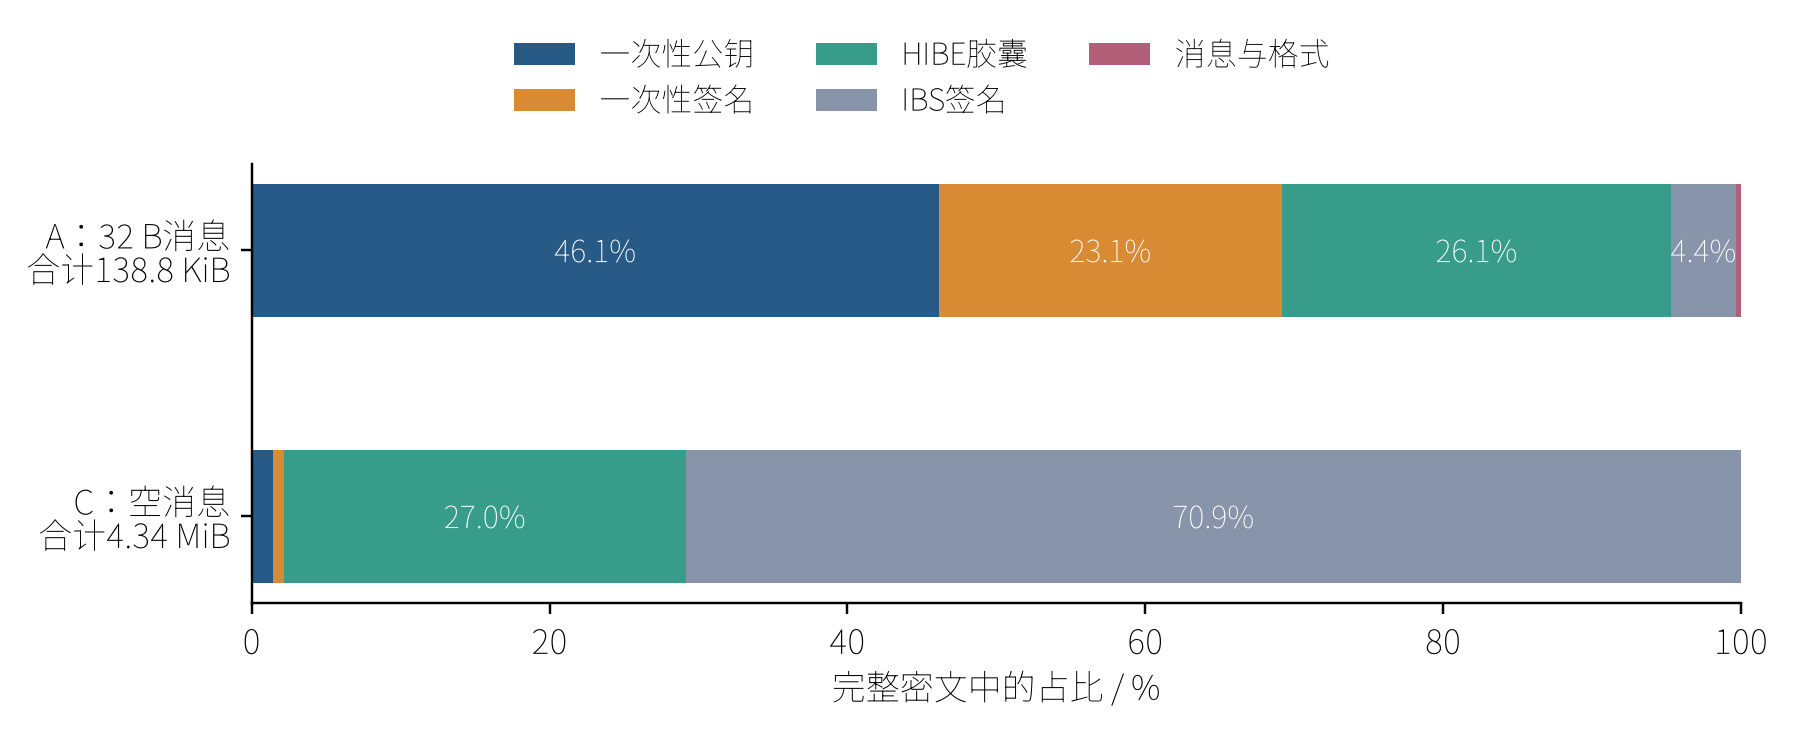
\includegraphics[width=.98\textwidth]{figures/ciphertext-parts.png}
\caption{完整密文的主要成本来源：A以一次性认证为主，C以IBS签名和HIBE胶囊为主}
\label{fig:ciphertext-parts}
\end{figure}

Lamport一次性公钥含1,024个64字节哈希像，签名含512个64字节原像，两项合计固定96 KiB，约占这条A密文的69.2\%。因此，缩短几字节应用消息几乎不会改变A的整包长度。C的IBS签名约占70.9\%，HIBE胶囊约占27.0\%；其后续通信优化应优先考察这两部分。

这也解释了SRGG签名紧凑编码与完整B密文的关系：签名字段变短会减少对称载荷，但整包还包含与A相同的一次性认证结构和LATTE胶囊。评价编码时应同时看单体对象与完整协议中的占比。

\subsection{消息长度与可用容量}
安装运行测试已完成A的0、32、1,024和59,191字节消息，B的0、32、1,024和65,364字节消息；超过应用上限1字节时，系统在生成新密文前拒绝。该批最大长度密文约为197 KiB和210 KiB。

C已完成空消息和1,024字节消息，两条密文相差1,024字节，符合固定胶囊与签名加上可变应用载荷的组成。C的3,924字节上限来自容量计算，尚缺该最大长度的加密解密记录。上述容量检查使用签名保守上界，具体签名和胶囊的编码长度仍可能随随机输出变化。

\section{三项主要优化的实验结果}
\subsection{Sageloli结构化采样结果}
Sageloli两个参数档均完成建立、身份发钥、两次签名和验证。表~\ref{tab:sageloli-times}给出各档一套系统的运行记录。

\begin{table}[H]
\centering\small
\caption{Sageloli结构化实现的实际运行，时间单位为秒}
\label{tab:sageloli-times}
\begin{tabular}{@{}lrrrrrr@{}}
\toprule
\rowcolor{black!8} 参数档 & 建立 & 发钥 & 首次签名 & 后续签名 & 验证 & RSS/GiB \\
\midrule
% BEGIN DATA sageloli-times.tex
PARAM-I & 4.99 & 85.1 & 9.28 & 2.02 & 0.517 & 1.36 \\
PARAM-II & 43.6 & 520 & 38.6 & 5.02 & 1.36 & 6.19 \\
% END DATA sageloli-times.tex
\bottomrule
\end{tabular}
\end{table}

PARAM-I发钥约85.1秒，记录峰值RSS约1.36 GiB；PARAM-II发钥约520秒，约6.19 GiB。首次签名
明显高于第二次，与同一身份陷门下数值计划可以复用的实现结构相符。两档参数都完成采样和公开
验证。第五章的1.18~TiB是稠密矩阵表示的理论存储量估算，本表记录的是未展开该矩阵的结构化
实现，因此二者分别说明原始瓶颈与实际资源占用。

\subsection{SRGG紧凑编码结果}
图~\ref{fig:codec}和表~\ref{tab:codec-sizes}展示三档SRGG相同数学对象的两种编码。每档独立建立3套系统，在同一对象上交替执行两种格式的编解码。

\begin{figure}[H]
\centering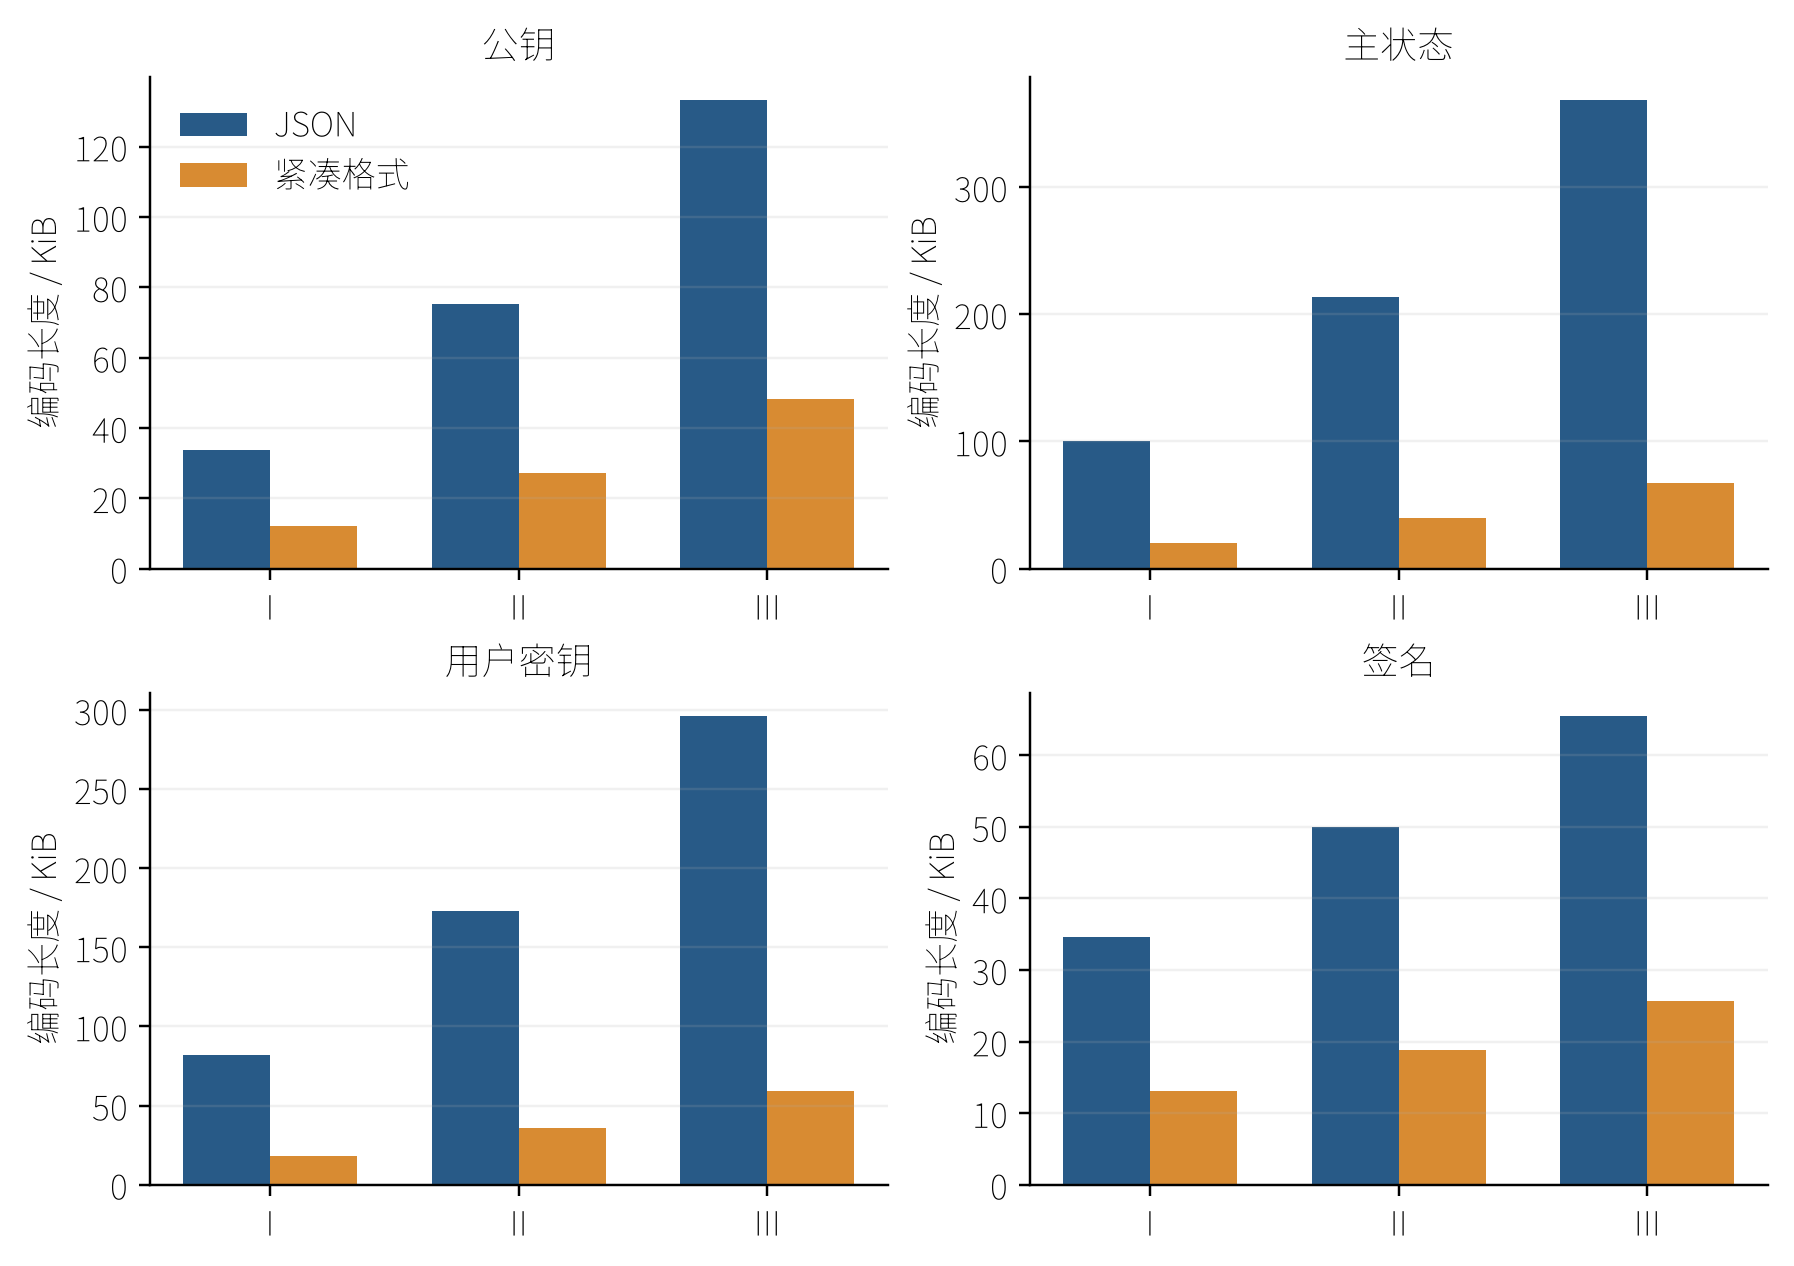
\includegraphics[width=.96\textwidth]{figures/codec.png}
\caption{SRGG三档参数的四类对象尺寸；I、II、III表示参数档}
\label{fig:codec}
\end{figure}

\begin{table}[H]
\centering\small
\caption{SRGG对象编码长度，单位为KiB}
\label{tab:codec-sizes}
\begin{tabular}{@{}lrrrr@{}}
\toprule
\rowcolor{black!8} 参数档／格式 & 公钥 & 主状态 & 用户钥 & 签名 \\
\midrule
% BEGIN DATA codec-sizes.tex
I／JSON & 33.7 & 100 & 82.2 & 34.5 \\
I／紧凑 & 12.1 & 19.8 & 17.8 & 13.1 \\
II／JSON & 75.2 & 213 & 173 & 49.9 \\
II／紧凑 & 27.1 & 40.1 & 35.6 & 18.8 \\
III／JSON & 133 & 368 & 296 & 65.5 \\
III／紧凑 & 48.1 & 67.5 & 59.5 & 25.6 \\
% END DATA codec-sizes.tex
\bottomrule
\end{tabular}
\end{table}

紧凑格式下，公钥占相应JSON长度的35.9\%至36.2\%，主状态占18.3\%至19.8\%，用户密钥占
20.1\%至21.7\%，签名占37.7\%至39.1\%。主状态中小范围陷门系数所占比例较高，按实际取值
范围位打包后，长度降幅最明显。

空间收益伴随位打包和规范检查的时间成本。以PARAM-I主状态为例，紧凑编码、解码中位时间约为
23.1毫秒和61.3毫秒，JSON编码、解码约为0.974毫秒和37.3毫秒。对于主状态保存、角色密钥
传递和签名传输，长度下降带来的收益更直接；高频内存内转换则需要同时考虑额外处理时间。

\subsection{Lai接收会话结果}
Lai会话实验使用一套主密钥，原路径解密2次，建立会话1次，会话内解密3次。原解密中位数为526秒，会话准备约510秒，后续解密中位数为28.6秒，额外保留叶钥编码34.7 MiB。

\begin{figure}[H]
\centering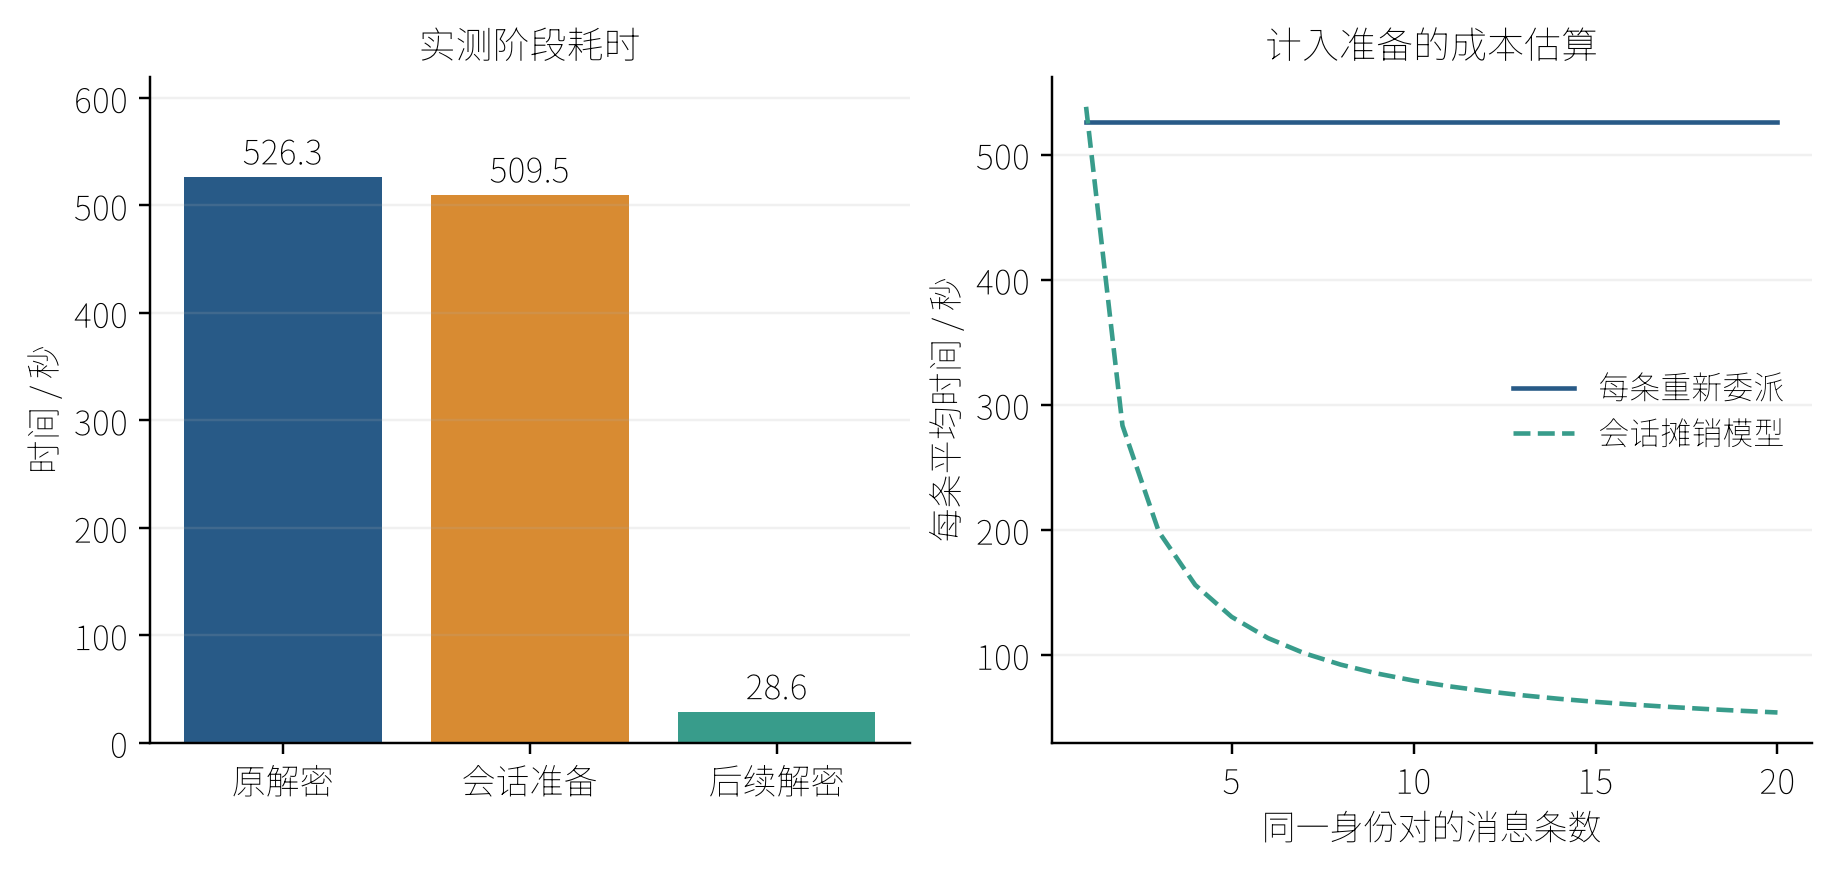
\includegraphics[width=.98\textwidth]{figures/session.png}
\caption{Lai接收会话：左图为测得阶段耗时，右图由阶段中位数代入成本公式估算}
\label{fig:session}
\end{figure}

准备完成后的单条时间约为原路径的$1/18.4$。把准备计入后，首条平均成本约538秒；按$\bar T(N)$模型，处理10条和100条消息时约为79.5秒和33.7秒。右图使用已有阶段耗时外推消息数量，未逐条执行整条曲线。

会话方法把主要委派开销移到首次使用，适合固定身份对的连续消息。短暂的一次通信仍要承担完整准备；长期会话则以额外秘密状态换取较低的后续延迟。该组样本来自一套系统，后续扩大测量可进一步观察不同主密钥下的波动。

\section{缓存与部署位置的完整流程对照}
\subsection{局部缓存对总耗时的影响}
在A、B各3套系统中，分别开启和关闭优化，以相同输入执行完整流程。A缓存机构证书的成功验证结果，原生验签调用由每条2次减少为1次，解密时间比中位数为1.086，逐套范围0.992至1.339。B复用签名数值准备，加密时间比中位数1.030，范围1.009至1.921。

这些结果说明，减少一次局部调用后，总时间仍受其余密码运算与运行波动影响。A有一套测量略微回退，B的中位收益较小。因此，系统保留缓存容量与关闭选项，主要优化结论仍以结构表示、编码和Lai会话为重点。

\subsection{文件部署位置对运行时间的影响}
三路部署对照固定参数、状态和原生引擎，均由同一WSL Python运行，分别使用Windows盘源码、Windows盘安装包及Linux盘同一安装包。每路完成30次完整加密和30次解密，图~\ref{fig:placement}给出中位数。

\begin{figure}[H]
\centering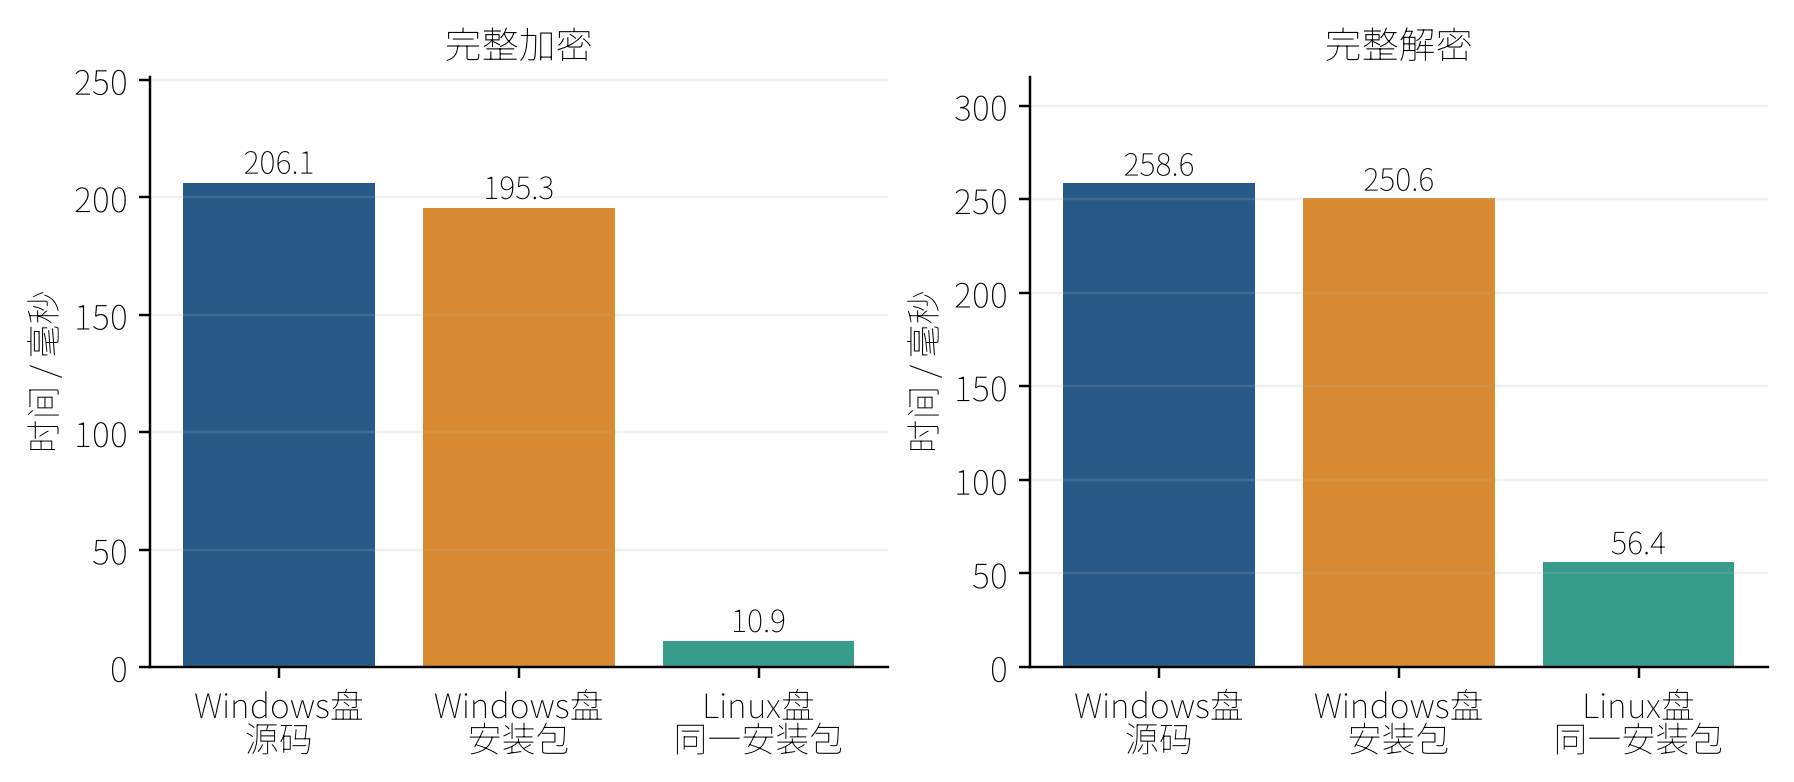
\includegraphics[width=.98\textwidth]{figures/placement.png}
\caption{文件放置位置对完整A流程的影响；三路均使用同一WSL运行时}
\label{fig:placement}
\end{figure}

Linux本地安装包的加密、解密中位时间分别为Windows盘源码运行的5.30\%和21.8\%。排除源码与
安装包差异，只比较同一安装包的两种位置时，相应比例为5.59\%和22.5\%。剖析记录中，5次加密
产生的515次文件读取在挂载目录累计约1.073秒，在Linux本地约0.011秒，说明文件访问是该批
运行的重要成本。因此，WSL部署优先把安装包和运行状态置于Linux本地文件系统。

\section{功能测试结果}
十组合同机实验中，每组均通过2次诚实加密、3次诚实解密、1次新进程恢复，以及截断和单比特
翻转两项外层拒绝，合计20次加密、30次解密、10次恢复和20次拒绝。更完整的异常语义由三组
代表实验覆盖：三组均完成双方匹配恢复、三类身份错配和多种字节异常拒绝。表
~\ref{tab:functional}汇总主要检查；另有A的随机身份与消息批次，独立建立3套系统、测试12组输入，
60/60项判断符合预期。

\begin{table}[H]
\centering\small
\caption{三组完整协议的主要功能结果}
\label{tab:functional}
\begin{tabularx}{\textwidth}{@{}Xccc@{}}
\toprule
\rowcolor{black!8} 检查情况 & A & B & C \\
\midrule
双方身份匹配 & 恢复原文 & 恢复原文 & 恢复原文 \\
仅接收身份不匹配 & 拒绝 & 拒绝 & 拒绝 \\
仅期望发送身份不匹配 & 拒绝 & 拒绝 & 拒绝 \\
双方身份都不匹配 & 拒绝 & 拒绝 & 拒绝 \\
密文字节修改、截断、追加或重复字段 & 拒绝 & 拒绝 & 拒绝 \\
外层认证有效、内部签名无效 & 拒绝 & 拒绝 & 拒绝 \\
新进程加载对象后解密 & 成功 & 成功 & 成功 \\
\bottomrule
\end{tabularx}
\end{table}

身份错配测试覆盖接收者、发送者和双方同时错误，分别触发不同层次的拒绝。密文字节修改、截断、
追加和重复字段覆盖外层认证与规范解析；“外层认证有效、内部签名无效”则单独检查IBS身份认证。
新进程恢复测试重新加载公开对象和角色密钥，再对已有密文解密，覆盖持久对象的完整使用路径。

\section{本章小结}

十种常规组合在统一机器、输入和运行配置下全部完成。横向结果表明，HIBE主要决定接收状态、胶囊
长度和解密委派，IBS主要决定发送者发钥、签名生成和发送钥尺寸。A的在线收发处于毫秒级；B的
主要时间集中在发送端SRGG签名，接收端仍为亚秒级；C的主要时间集中在Lai叶钥委派。Wang--PW
的Setup、发钥和签名需要服务器级资源，但接收端解密保持在数秒量级。

通信量分析表明，A的密文主要由一次性认证构成，C主要由IBS签名和HIBE胶囊构成。对象级优化
能否明显缩短完整密文，取决于目标字段在整包中的占比。功能测试与恢复测试进一步确认，同一套
协议在A、B、C以及十种常规组合中保持一致的身份匹配和字节处理流程。三项主要优化分别降低了
Sageloli采样内存、SRGG对象尺寸和Lai连续解密延迟。

\chapter{创新性与应用前景}

本作品以“多类格原语能否组成同一套可运行IB-ME系统”为主线，在统一协议中实现多种HIBE与
IBS，并针对不同后端的主要瓶颈完成结构化计算、紧凑编码和会话复用。本章先归纳作品在通用
设计、算法实现和工程优化方面的创新，再结合三组代表的性能特点分析适用场景与部署方式。

\section{作品创新性概述}

作品的创新并非来自单一算法替换，而是从协议组合、软件实现和运行优化三个层次建立联系。
表~\ref{tab:innovation-summary}按照“问题、方法、结果、适用条件”归纳主要工作。

\begin{table}[H]
\centering\small
\caption{作品主要创新及其实际效果}
\label{tab:innovation-summary}
\begin{tabularx}{\textwidth}{@{}>{\raggedright\arraybackslash}p{.18\textwidth}>{\raggedright\arraybackslash}p{.25\textwidth}>{\raggedright\arraybackslash}p{.27\textwidth}>{\raggedright\arraybackslash}X@{}}
\toprule
\rowcolor{black!8} 面向的问题 & 采用的方法 & 已实现结果 & 适用条件 \\
\midrule
格HIBE与格IBS的对象、参数和容量差异较大
& 稳定原语接口、能力声明、规范编码与组合预检
& 两种HIBE、五种常规IBS形成十种组合，完成同机比较并接入Wang--PW目标档
& 新后端需实现接口、对象编解码、能力声明与原语自检 \\

Sageloli目标参数不能展开完整相关扰动矩阵
& 保留环多项式结构，逐频率分解低秩Gram矩阵
& PARAM-I、II均完成发钥、签名和公开验证，峰值RSS分别约1.36、6.19~GiB
& 数值计划与最终精确模方程分别检查 \\

SRGG参考JSON对象含有大量文本和结构开销
& 按字段取值范围定长编码，并检查唯一表示
& 三档主状态为JSON长度的18.3\%至19.8\%，签名为37.7\%至39.1\%
& 以额外编解码时间换取存储和传输长度下降 \\

Lai固定身份对通信会重复执行二级委派
& 建立绑定公钥及双方身份的接收会话，复用叶密钥
& 准备约510秒后，后续解密中位数为28.6秒
& 适合固定身份对的连续消息，并额外保留34.7~MiB叶密钥 \\

大对象矩阵SIS IBS难以进入统一应用流程
& 流式保存用户陷门，将目标档后端接入现有LATTE组合
& 完成目标规模建立、发钥、独立签名、公开验签和完整组合收发
& 发钥与发送端需要服务器级内存，适合低频或离线任务 \\
\bottomrule
\end{tabularx}
\end{table}

第一项工作体现“通用设计”：公共五算法、传输格式、状态管理和应用入口不依赖某一种矩阵或环
表示。后三项工作体现“优化实现”：先从完整流程中识别主要成本，再依据相应算法的结构改变计算
或数据组织。Wang--PW接入则进一步检验接口能否容纳远大于常规方案的密钥和签名对象。

\section{应用需求与方案选择}

IB-ME适合“发送给某个身份，并要求只有认可特定发送身份的接收者才能恢复”的通信。与只检查
接收地址的加密相比，它把发送身份条件纳入密钥恢复；与先解密再验签的简单串联相比，接收者在
恢复过程中同时使用接收身份和期望发送身份。实际部署时，还要根据交互延迟、发送端资源、通信
频率和状态保存条件选择具体组合。

\begin{table}[H]
\centering\small
\caption{代表方案与应用需求的对应关系}
\label{tab:application-choice}
\begin{tabularx}{\textwidth}{@{}>{\raggedright\arraybackslash}p{.22\textwidth}>{\raggedright\arraybackslash}p{.2\textwidth}>{\raggedright\arraybackslash}p{.24\textwidth}>{\raggedright\arraybackslash}X@{}}
\toprule
\rowcolor{black!8} 主要需求 & 建议组合 & 选择依据 & 使用条件 \\
\midrule
交互式定向消息、现场演示 & A：LATTE＋BNN／ML-DSA & 同机重复加密、解密为13.5、59.4毫秒 & 可接受约139~KiB固定密文开销 \\
原生模格身份签名与紧凑状态 & B：LATTE＋SRGG & 同机重复加密11.3秒，重复解密68.7毫秒 & 发送者发钥和签名适合预先或异步执行 \\
固定身份对的连续通信 & C：Lai＋Sageloli & 完整重复解密409秒；专项会话实验降至28.6秒 & 通信双方稳定，能够保留会话叶密钥 \\
低频、目标规模矩阵SIS任务 & LATTE＋Wang--PW & 完成大对象后端的完整协议接入 & 发送端具备服务器级内存，密钥预先生成 \\
\bottomrule
\end{tabularx}
\end{table}

该对应关系不是把组合划分为互不相容的产品，而是说明统一框架能够按照部署条件选择后端。应用
接口、身份语义和密文字节格式保持一致，变化集中在参数、对象尺寸和运行资源。

\section{机构定向消息与跨部门协作}

在单位内部，通知、审批结果、值班指令和受控资料通常具有明确的发送部门和接收岗位。以“安全
管理部门向区域值班负责人发送临时处置指令”为例，发送端以部门身份取得IBS签名密钥，接收端
以岗位身份取得HIBE一级密钥。加密时指定岗位身份，接收时再指定认可的部门身份；只有两项均与
密文一致时才能恢复正文。

这一模式可以减少传统证书目录查询和逐用户公钥分发的工作。人员变动时，系统可以把部门、岗位、
有效期或组织层级编码进身份字符串，由发钥机构按现有组织目录签发角色对象。跨部门协作时，
双方仍需共享同一套公开参数和身份编码规则，但不必在每次通信前交换临时公钥。

对于需要即时反馈的消息，A组的在线时间更适合交互式客户端。若发送任务由后台队列执行，且
希望使用原生模格IBS及更紧凑的状态文件，可选B组。系统已有命令行和浏览器入口，实际集成时
还可以把规范密文字节放入现有消息队列、文件交换或数据库字段中。

\begin{figure}[H]
\centering
\begin{tikzpicture}[node distance=7mm and 13mm]
 \node[check,text width=35mm] (issuer) {机构发钥服务\\签发部门与岗位密钥};
 \node[flow,below left=of issuer,text width=37mm] (sender) {发送部门\\指定接收岗位并加密};
 \node[flow,below right=of issuer,text width=37mm] (receiver) {接收岗位\\指定认可发送部门};
 \node[check,below=of issuer,yshift=-36mm,text width=42mm] (transport) {现有业务通道\\传递规范IB-ME密文};
 \node[check,below=of transport,text width=42mm] (result) {双方身份同时匹配\\恢复并处理业务消息};
 \draw[flowarrow](issuer)--node[left,font=\small]{发送密钥}(sender);
 \draw[flowarrow](issuer)--node[right,font=\small]{接收密钥}(receiver);
 \draw[flowarrow](sender)--(transport);
 \draw[flowarrow](transport)--(receiver);
 \draw[flowarrow](receiver)--(result);
\end{tikzpicture}
\caption{机构定向消息中的身份签发与密文流转}
\label{fig:institutional-message}
\end{figure}

\section{受控终端与设备指令分发}

管理平台向终端设备发送配置、更新通知或控制指令时，接收方不仅要确认消息发给本设备或本设备组，
还要限制可以被接受的管理身份。可以把设备编号、区域和用途组织为接收身份，把管理域或控制服务
名称组织为发送身份。终端只为预先认可的管理身份派生叶密钥，从而在协议层表达“发给哪台设备、
由哪个管理域发出”两个条件。

设备场景的选择取决于运行方式。偶发指令强调单次响应，可优先考虑A组；同一管理端持续向固定
设备发送多条数据时，可以在资源允许的网关或边缘节点使用C组会话，将二级委派安排在连接建立
阶段。对于存储受限终端，当前Lamport一次性认证带来的固定96~KiB开销仍需进一步优化，因此更
适合由网关承担密码处理，而不是直接部署到极小型传感器。

\section{固定身份对的连续通信}

远程运维、跨域数据同步和周期性报送通常在较长时间内保持双方身份不变。C组的特点正是把昂贵
的Lai委派从每条消息移到会话准备阶段。接收端在连接建立时生成$(r,s)$叶密钥并完成绑定检查，
后续每条消息继续执行字节认证、HIBE解封装、对称认证与IBS验签。

这类应用应把会话生命周期与业务连接对齐：更换发送身份、接收身份、公开参数或组合配置时重新
准备；连接结束后释放叶密钥；长期身份密钥仍由固定发钥服务管理。第七章的摊销模型表明，消息
数量越多，单条平均成本越接近会话内解密时间。若只传送一条消息，会话并不能减少首次总成本，
此时应根据延迟要求选择A或B。

\section{密码迁移与算法扩展}

后量子迁移不仅是把一种算法替换成另一种算法，还要处理参数、对象格式、密文容量和运行依赖的
变化。作品把这些差异放入后端能力声明和组合配置，使应用层能够在建立系统前得到身份长度、
载荷容量、签名上界和依赖检查结果。新增HIBE可以与现有IBS逐一配对，新增IBS也可以复用现有
HIBE、五算法、状态文件、命令行和网页流程。

这种结构适合作为算法评测与迁移原型。一方面，同一完整协议可以比较不同困难问题、参数档和
编码方法的实际代价；另一方面，应用可以先以低延迟组合完成业务接入，再根据部署资源切换到
其他后端，而不改变双方身份含义和操作顺序。第四章的组合矩阵和Wang--PW接入已经展示了两种
扩展方向。

\section{应用部署的实施条件}

从原型进入实际业务还需要完成身份治理、密钥保护、运行审计和统一环境测量。身份编码应与组织
目录、设备台账或业务角色保持一致，并明确有效期与撤销策略；发钥机构的主状态应部署在受控环境，
用户密钥应按角色分发；服务端任务需要记录组合版本、参数摘要和失败原因，但不记录主秘密或消息
明文。

十种常规组合已经在Ultra~9~275HX上以相同源码、运行时、线程配置、身份长度和消息长度完成
同机基本比较，部署选型可以先依据第七章的完整时间、对象尺寸与内存数据，再结合目标业务决定
离线准备和会话复用方式。该批每种组合只有一个独立根，适合判断成本量级和主要瓶颈；若要评估
运行波动，还应参考A/B多根实验，并在目标服务器上增加重复测量。Wang--PW使用128~GiB级服务器
分阶段运行，继续作为资源型后端单独评估，不与十种常规组合直接排名。

\section{本章小结}

作品的应用价值来自统一身份语义下的多算法选择能力。A面向低延迟定向消息，B面向原生模格认证
和紧凑状态，C面向固定身份对的连续通信，Wang--PW则补充目标规模矩阵SIS后端。机构消息、设备
指令和跨域连续通信都可以使用同一五算法与传输格式，再根据发送端资源、通信频率和状态条件选择
具体组合。

\chapter{总结与展望}

\section{工作总结}

本作品围绕“基于多类格困难假设的抗量子身份基匹配加密通用设计和优化实现”完成了从理论构造、
密码原语到应用入口的完整实现。系统以两层匿名HIBE承载接收身份和认可发送身份，以IBS认证
发送者，并通过短种子混合加密承载不同长度的应用消息。完整密文进一步绑定一次性验签公钥和
全部传输字节，使身份条件、载荷与外层字节认证处于同一处理流程。

在算法层，作品实现LATTE、Lai两种HIBE，以及BNN＋ML-DSA、BNN＋Falcon、Luo、SRGG、
Sageloli五种常规IBS，形成十种端到端组合；在此基础上又接入Wang--PW目标参数矩阵SIS后端。
三组代表分别覆盖低延迟交互、原生模格身份签名和固定身份对连续通信。所有组合复用相同的公共
五算法、对象边界、状态管理、命令行和浏览器入口。

在优化层，作品针对完整运行中出现的主要瓶颈提出三项实现方法：Sageloli结构化采样保留环结构，
把大规模相关扰动转化为逐频率低秩计算；SRGG范围感知编码按字段实际取值范围压缩四类对象；
Lai接收会话复用固定身份对的叶密钥，将重复委派移到准备阶段。三项优化都不改变相应算法的
公开方程，也不要求修改通用IB-ME协议。

在软件层，后端通过稳定接口、能力声明和规范编解码接入。组合预检在建立系统前确认身份宽度、
签名输入、载荷容量、对象格式和运行依赖；固定发钥服务与原子状态保存支持跨进程恢复；CLI和
Web界面完成密钥建立、角色导出、定向加密、匹配解密及错误输入演示。

\section{实验结论}

A组重复加密、解密中位数分别为78.5毫秒和152毫秒，适合交互式演示和定向消息。B组的主要
时间集中在发送者发钥和SRGG签名，重复解密中位数为161毫秒；三档SRGG主状态的紧凑长度为
JSON的18.3\%至19.8\%，说明字段范围对大对象存储具有明显影响。

C组一次完整解密中，Lai委派约占92.5\%。接收会话把该阶段前移后，会话准备约510秒，后续
解密中位数为28.6秒。Sageloli PARAM-I、II均完成目标参数发钥、签名和公开验证，结构化实现
的峰值RSS分别约1.36~GiB和6.19~GiB。Wang--PW完成目标规模建立、身份发钥、独立签名、公开
验签及LATTE组合，其大对象和服务器级资源需求也说明通用接口需要同时容纳轻量与重型后端。

密文组成分析表明，A组主要开销来自Lamport一次性认证，C组主要开销来自Sageloli签名和Lai
胶囊。优化单个对象能否显著改变完整传输量，取决于该对象在整包中的占比。身份错配、字节篡改、
截断、追加、内部签名错误和跨进程恢复测试则覆盖了统一协议的主要功能路径。

\section{后续工作}

第一项后续工作是在Ultra~9~275HX同一机器上完成十种常规组合补测。统一操作系统、Python与
Sage版本、线程配置、身份长度、消息长度和重复次数后，可以形成更严格的组合横向对比，并补充
时间分位数、进程树峰值内存、对象尺寸和完整密文长度。

第二项工作是降低协议级固定通信开销。当前Lamport一次性公钥与签名合计96~KiB，在A组短消息
中占据主要比例。后续可研究更紧凑的一次性认证或直接采用具备所需强不可伪造性质的签名构造，
同时保持完整密文字节绑定和现有错误输入语义。

第三项工作是继续扩展HIBE与IBS后端。接入过程已经固定为接口实现、能力声明、规范编解码、
原语自检和组合测试；后续可以增加其他环格、模格或矩阵格方案，并在同机条件下比较它们在
Setup、发钥、在线收发、持久恢复和通信量方面的差异。

第四项工作是完善面向长期部署的身份与密钥管理，包括带有效期的身份编码、密钥撤销与更新、
硬件隔离的主状态、会话密钥清理和运行审计。浏览器演示已经验证角色操作流程，进一步集成时可
将规范密文字节接入现有消息队列或文件交换系统，并保持密码运算与业务界面的分层。

通过这些工作，系统可以从多算法研究原型继续发展为可复现、可扩展并适应不同资源条件的后量子
身份基匹配加密平台。


\clearpage
\addcontentsline{toc}{chapter}{参考文献}
\begin{thebibliography}{99}
\small

\bibitem{shor1994}
Peter W. Shor.
Algorithms for Quantum Computation: Discrete Logarithms and Factoring.
In \emph{Proceedings of the 35th Annual Symposium on Foundations of Computer Science},
pp. 124--134, 1994.

\bibitem{shamir1984}
Adi Shamir.
Identity-Based Cryptosystems and Signature Schemes.
In \emph{Advances in Cryptology---CRYPTO 1984}, LNCS 196, pp. 47--53, 1985.

\bibitem{bonehfranklin2003}
Dan Boneh and Matthew Franklin.
Identity-Based Encryption from the Weil Pairing.
\emph{SIAM Journal on Computing}, 32(3), pp. 586--615, 2003.

\bibitem{gentrysilverberg2002}
Craig Gentry and Alice Silverberg.
Hierarchical ID-Based Cryptography.
In \emph{ASIACRYPT 2002}, LNCS 2501, pp. 548--566, 2002.

\bibitem{hess2003ibs}
Florian Hess.
Efficient Identity Based Signature Schemes Based on Pairings.
In \emph{Selected Areas in Cryptography 2002}, LNCS 2595, pp. 310--324, 2003.

\bibitem{ajtai1996}
Miklós Ajtai.
Generating Hard Instances of Lattice Problems.
In \emph{Proceedings of the 28th Annual ACM Symposium on Theory of Computing},
pp. 99--108, 1996.

\bibitem{regev2005lwe}
Oded Regev.
On Lattices, Learning with Errors, Random Linear Codes, and Cryptography.
In \emph{Proceedings of the 37th Annual ACM Symposium on Theory of Computing},
pp. 84--93, 2005.

\bibitem{wang2024ibme}
Yuejun Wang, Baocang Wang, Qiqi Lai, and Yu Zhan.
Identity-based Matchmaking Encryption with Stronger Security and Instantiation on Lattices.
\emph{Theoretical Computer Science}, 2024.
doi: 10.1016/j.tcs.2024.115048.

\bibitem{zhao2024latte}
Raymond K. Zhao, Sarah McCarthy, Ron Steinfeld, Amin Sakzad, and Máire O'Neill.
Quantum-safe HIBE: Does It Cost a LATTE?
\emph{IEEE Transactions on Information Forensics and Security}, 2023.

\bibitem{lai2015trapdoors}
Russell W. F. Lai, Henry K. F. Cheung, and Sherman S. M. Chow.
Trapdoors for Ideal Lattices with Applications.
In \emph{Inscrypt 2014}, LNCS 8957, pp. 239--256, 2015.
doi: 10.1007/978-3-319-16745-9\_14.

\bibitem{jia2025ibs}
Huiwen Jia, Ying Liu, Chunming Tang, and Lin Wang.
Constructing Efficient Identity-Based Signatures on Lattices.
\emph{IET Information Security}, 2025.
doi: 10.1049/ise2/6684889.

\bibitem{sageloli2023ibs}
Éric Sageloli, Pierre Pébereau, Pierrick Méaux, and Céline Chevalier.
Shorter and Faster Identity-Based Signatures with Tight Security in the (Q)ROM from Lattices.
In \emph{ACNS 2023}, 2023.
doi: 10.1007/978-3-031-33488-7\_24.

\bibitem{pan2021ibs}
Jiaxin Pan and Benedikt Wagner.
Short Identity-Based Signatures with Tight Security from Lattices.
In \emph{PQCrypto 2021}, 2021.
ePrint 2021/970.

\bibitem{galindo2006ibs}
David Galindo, Javier Herranz, and Eike Kiltz.
On the Generic Construction of Identity-Based Signatures with Additional Properties.
In \emph{ASIACRYPT 2006}, 2006.

\bibitem{nist2024fips204}
National Institute of Standards and Technology.
\emph{Module-Lattice-Based Digital Signature Standard}.
FIPS 204, 2024.

\bibitem{micciancio2012trapdoors}
Daniele Micciancio and Chris Peikert.
Trapdoors for Lattices: Simpler, Tighter, Faster, Smaller.
In \emph{EUROCRYPT 2012}, 2012.

\bibitem{lpr2013ring}
Vadim Lyubashevsky, Chris Peikert, and Oded Regev.
On Ideal Lattices and Learning with Errors over Rings.
\emph{Journal of the ACM}, 60(6), 2013.

\bibitem{langlois2015module}
Adeline Langlois and Damien Stehl\'e.
Worst-Case to Average-Case Reductions for Module Lattices.
\emph{Designs, Codes and Cryptography}, 75, pp. 565--599, 2015.

\bibitem{rfc5869}
Hugo Krawczyk and Pasi Eronen.
HMAC-based Extract-and-Expand Key Derivation Function (HKDF).
RFC 5869, 2010.

\bibitem{nist2007gcm}
National Institute of Standards and Technology.
\emph{Recommendation for Block Cipher Modes of Operation: Galois/Counter Mode (GCM) and GMAC}.
Special Publication 800-38D, 2007.

\bibitem{lamport1979ots}
Leslie Lamport.
Constructing Digital Signatures from a One Way Function.
SRI International, CSL-98, 1979.

\bibitem{luo2024ibs}
Pingbin Luo, Xinjian Chen, Willy Susilo, and Qiong Huang.
Identity-Based Signature from Lattices without Trapdoors.
In \emph{ICICS 2024}, 2024.

\bibitem{falcon2020}
Pierre-Alain Fouque et al.
\emph{Falcon: Fast-Fourier Lattice-based Compact Signatures over NTRU}.
Specification v1.2, 2020.

\end{thebibliography}

\end{document}
